%%%%%%%%%%%%%%%%%%%%%%%%%%%%%%
%%%%%%%% Motivation %%%%%%%%%%
%%%%%%%%%%%%%%%%%%%%%%%%%%%%%%
\chapter{Motivation}
Nowadays machine learning and deep learning have become a distinguished approach for visual
recognition tasks and have achieved great success in this process. However, they require a large amount of
labeled data to learn. Providing this amount of labeled data does not only bring much effort along
but also occupies a huge amount of storage. In
contrast, we as humans are very good in visual recognition, so that we are able to learn with one or few\footnote{This is known as few-shot learning in
  deep learning and represents the scenario when there are one or few instances of each class in
  training-set to learn.}
examples. Imagine a child who is able to recognize a lion in a picture
after learning from, few examples, how lions look like. We want to simulate and apply this ability to deep learning
such that, few examples are sufficient to achieve a desirable accuracy.
In this bachelor thesis, we focus on few-shot learning in deep learning. We aim at
learning and training a model for a small set of labeled examples. We enlarge our dataset by
generating artificial examples based on the examples at hand. This technique is known as data
augmentation. These artificial labeled examples help to increase accuracy and prevent overfitting. Data augmentation is our focus in this work to achieve few-shot
learning and prevent overfitting. In the following, we will introduce several well-known techniques
of data augmentation. The first purpose will be to discover if and how far data augmentation can
improve the learning process and accuracy. The second step will be to compare their accuracy. In
the end, we aim at discovering potential combinations of different approaches and techniques of data
augmentation to increase accuracy and reduce the error-rate.
We will focus on visual recognition tasks and their classification. Additionally, we will
concentrate on the implementation of various techniques of data augmentation for convolutional
neural networks.


%%%%%%%%%%%%%%%%%%%%%%%%%%%%%%
%%%%%%%% Introduction %%%%%%%%
%%%%%%%%%%%%%%%%%%%%%%%%%%%%%%
\chapter{Introduction}
Neural networks can possibly contain multiple non-linear layers which makes them very expressive models
that are able to learn complex relationships between input and output parameters. Even with limited
input data, neural networks discover and learn many relations from the data. However, sometimes the
discovered and learned relations do not exist or  consist of redundant information and
relations. Redundant relations potentially arise from data-noise or lack of data-generalization.
Non-existent relations can potentially emerge from lack of sufficient data. These phenomena are known as
\textit{overfitting} in deep learning. In other words, learning with few labeled examples or noisy
data causes overfitting. Overfitting causes low accuracy and high error-rates. Hence, our goal is to
propagate from artificial labeled examples from a few given examples to prevent overfitting and reduce the error-rate and increase
the accuracy.

As we mentioned acquiring a huge labeled dataset is expensive and seeks much effort and time.
Therefore, we aim to generate artificial examples from few labeled examples. In other words, we
augment our data which is known as data augmentation. There are a few well-known techniques for data
augmentation. We will introduce the following techniques by implementing their strategy and
comparing their efficiency and capability:
\begin{itemize}
  \item \textbf{Image Translations} \ref{tit:image_translations}
  \item \textbf{Elastic Distortions} \ref{tit:elastic-distrotion}
  \item \textbf{Stroke Warping} \ref{tit:stroke-warping}
  \item \textbf{Bayesian Approach} \ref{tit:bayesian-approach}
\end{itemize}


%%%%%%%%%%%%%%%%%%%%%%%%%%%%%%
%%%%%%% Data Augmentation %%%%%
%%%%%%%%%%%%%%%%%%%%%%%%%%%%%%
\chapter{Data Augmentation}
\label{tit:data-augmentation}
In this chapter, we will introduce a few noteworthy related works in this field which mainly consist
of two approaches and several techniques.
In what follows, we solely focus on image data.  While some techniques might be applicable to other
types of data as well, we shall explore them when used on image datasets.

As the name clears itself, we are looking for enlarging datasets artificially and generate synthetic
data based on the obtainable few samples to increase the accuracy of the prediction.

\section{Label Preserving Transformations}
When training neural networks, label preserving transformations are a commonly used approach with classes of
techniques for enlarging datasets by generating generic data. The advantage of using this approach
and its techniques, when available, is twofold. The first benefit is the low space complexity of these
methods since one does not necessarily need to save the generated data on storage. Also, these
transformations are usually of relatively smaller time complexity compared to other approaches,
which makes them desirable in many instances in practice.

As the name may suggest, the ultimate goal when using these techniques is to generate synthetic data points after applying a set of suitable transformations to a real data point.

\subsection{Image Translations}
\label{tit:image_translations}
Image translation is one of the simplest and meanwhile applicable well-known technique of the label
preserving transformations approach. As the research by Krizhevsky et al.
\cite{image_translation_paper} proposes, we extract
image translations and their horizontal reflections to generate synthetic data and augment the
dataset. Image translation consists of extracting patches that are smaller in size than the original
image. Given a single channel (grayscale) $n \times n$ image and a translation patch of the size
$m$ for some $m<n$, one can produce $(n-m+1) \times (n-m+1) $ synthetic instances of the datapoint. Also, taking
the horizontal reflections of each newly generated data point into account, one can enlarge the
dataset by a factor of two, therefore finally the dataset can be enlarged by factor of:

\begin{equation}
  \label{eq:image_translate}
  2\times(n-m+1)\times(n-m+1)
\end{equation}

Figure \ref{fig:label-preserving-trasformation} is an illustration of the translations and horizontal
reflections of a $4 \times 4$ image, using all
possible patches of the size $3 \times 3$, which results in eight new data points.

At test (prediction) time, the method extracts the patches with the same size ($m < n$), however this time the
patches will be extracted from the four corners and the center of the test image. The network predicts on these
five patches and their horizontal reflections (ten patches altogether). In the end, the average
on the softmax layer will be determined by the final prediction.

\begin{figure}
  \centering
  \label{fig:label-preserving-trasformation}
  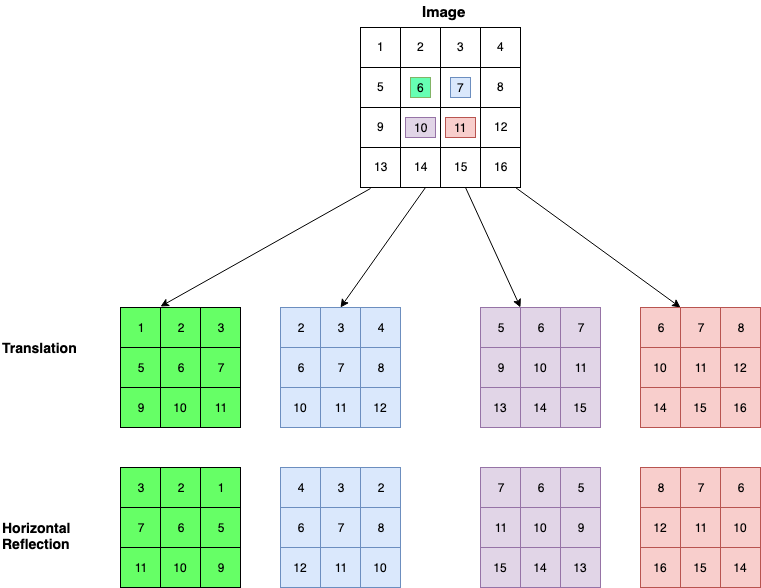
\includegraphics[width=1\textwidth]{fig/label-preserving-transformation}
  \caption{An example of single channel image with size of $4\times4$ with its translations with size of $3\times3$ patches and their horizontal reflections. The numbers determinate the pixels intensity.}
\end{figure}


\subsection{Elastic Distortions}
\label{tit:elastic-distrotion}
Another well-known technique for data augmentation is elastic distortion. Quite similar to image
translation, the ultimate goal is to generate synthetic dataset from a single data point. However, instead of
taking patches which are smaller than the original image, the synthetically produced data points are
of the same size as the original image as proposed by \cite{elastic_distortion_paper} . This is done by moving pixels and modifying pixel intensity
according to both their former and new position.  To this end, a few interpolation schemes such as
the nearest neighbor, bicubic, spline, and bilinear are available. Due to their practical
effectiveness and simplicity, we use the bilinear interpolation scheme in this work, which we
discuss in detail below.

Let $\alpha \in \mathbb{R}$, and let $\Delta x(x,  y) = \alpha x$ and $\Delta y(x,  y) = \alpha y$
denote the horizontal and the vertical displacement of a point $(x, y)$ of an image respectively.
Since the scaling parameter $\alpha$ could take a non-integer value, the interpolation task is
necessary for adjusting the intensity of pixels. Utilizing the bilinear interpolation, we adjust the
intensity of a shifted pixel according to its former location and intensity of its neighbors
therein. A formal description of the procedure is as follows. In what follow we will show and summarize the
process formally.

\begin{definition}{}
  Given the pixel $p'$. We want to displace it with $\Delta x(x,y)= \alpha x$. Let $\Delta y(x,y)= \alpha y$ and $p_{(x,y)}, p_{(x+1,y)}, p_{(x,y-1)}, p_{(x+1,y-1)}$ the neighbors (on
  origin square) of $p'$ in the new location after displacement and $I(p)$ shows the intensity of pixel $p$. Then the vertical interpolation yields:

  $$V_1 = I(p_{(x,y)}) + \big( \Delta x(p', p_{(x,y)}) \times I(p_{(x+1,y)}) \big)$$
  $$V_2 = I(p_{(x,y-1)}) + \big( \Delta x(p', p_{(x,y-1)}) \times I(p_{(x+1,y-1)}) \big)$$

  And then the horizontal interpolation yields a new intensity for pixel $p'$ after displacement:
  $$I(p') = V_1 + \big( \Delta y(p', p_{(x,y-1)}) \times V_2) \big)$$
\end{definition}

In practice, usually, one picks the scaling parameter $\alpha$ from the interval $[-1, 1]$ uniformly
at random. At the final stage of the procedure, the fields  $\Delta x(x,  y)$ and $\Delta y(x,  y)$
are convolved with a Gaussian filter with a standard deviation of $\sigma$, whose value depends on
the size and the entropy of the image. Observe that this technique is called the elastic distortion
mainly because the procedure described above results in an elastically deformed instance
of the original image.

Similar to image translation, at test (prediction) time, the image will be augmented by a factor of
ten with elastic distortion. Finally and in test and prediction time, average on softmax layer for
this enlarged ten images determines the prediction (label).

\subsection{Stroke Warping}
\label{tit:stroke-warping}
Similar to the previously introduced techniques, stroke warping uses predetermined families of transformations.
In other words, we enlarge our dataset artificially with the aid of well-known classical computer
vision transformations. This technique not withstanding of non-heavy complexity accomplished desirable
results even on medical purposes \cite{stroke_tumor}. The ideas of this technique are raised from Tangent
Dist \cite{stroke_idea_1992} and Tangent Prop \cite{stroke_idea_1993} works.

In this technique, we perform small changes in images to augment our data.  That means we augment our
images with skewing, rotating, and shearing (scaling) \cite{storke_warping_1997_source}. Similar to
image translation and elastic distortion the augmentation will be started before the
training phase and the training will be performed on enlarged data. Figure
\ref{fig:stroke_warping_transforamtions} represents each mentioned transformation to make them visually
understandable.

At test (prediction) time, the image will be enlarged by factor of ten and prediction will be performed on
averaging of softmax layer of ten  images, similar to the previous techniques.

\begin{figure}
  \centering
  \label{fig:stroke_warping_transforamtions}
  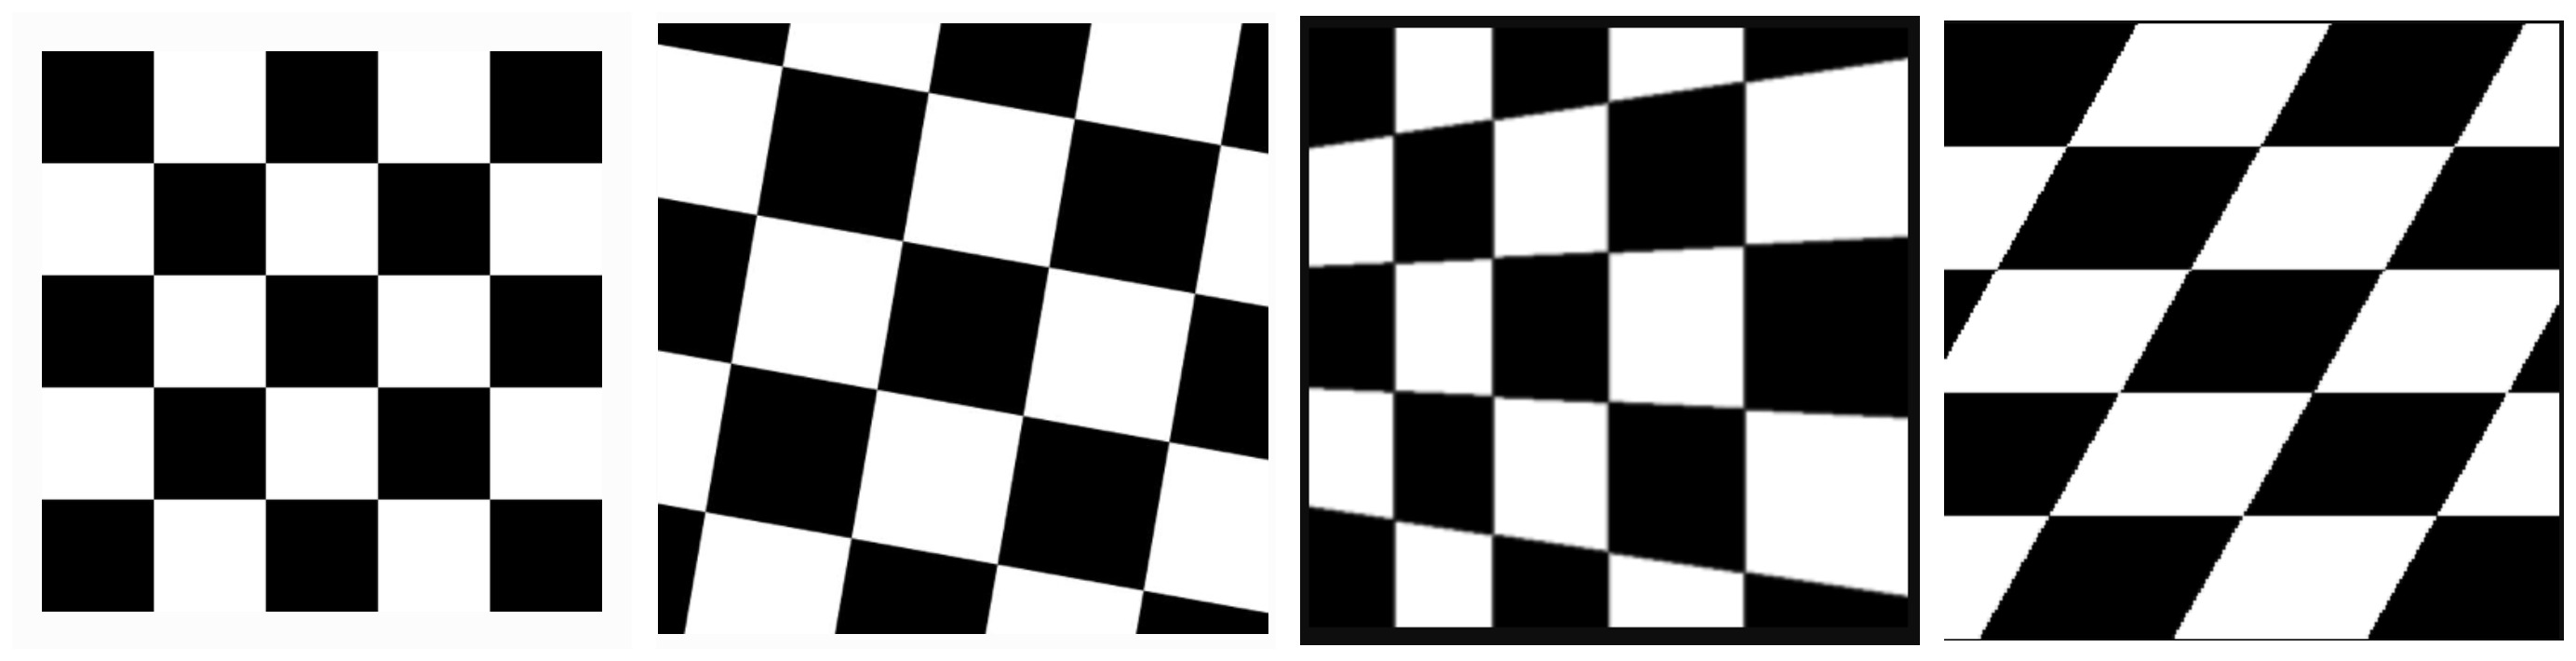
\includegraphics[width=1\textwidth]{fig/stroke_warping_transforamtions}
  \caption{An example of rotation, skew, and shear (scale) transformations for stroke warping \cite{stroke_warping_github_picture}.}
\end{figure}


\section{Bayesian Approach}
\label{tit:bayesian-approach}
The astute reader should have noticed that, although quite different, all the introduced techniques so far share a fundamental aspect. Precisely speaking, in all these techniques, one obtains new training samples by applying a set of predefined random transformations on the annotated training data, and the augmentation procedure ends before the training phase starts. This widely used process is called the poor man's data augmentation (PMDA) \cite{poor_man_data_augmentation}. However, to the best of our knowledge, this is not the furthest that one can go. Indeed, the fact that neural networks are generally capable of learning complicated patterns and nonlinear relationships in images suggests that they should also be able to learn latent variables so that they can enhance the data augmentation process dynamically.
In direct contrast to PMDA, in Bayesian data augmentation, the training set evolves dynamically and
in an iterative fashion during the training phase, which could considerably enhance the
generalization ability of a neural network. This approach uses a number of techniques to achieve this
matter as such as maximum a posterior probability (MAP) \cite{MAP_Bayesian} in Bayesian statistics and Generative
Adversarial Networks (GANs). Before diving directly into technical details about the
Bayesian data augmentation, we briefly introduce generative models. First, we
present the Generative Adversarial Networks (GANs) proposed initially by Goodfellow et al.
\cite{goodflew_bayesian_approach}. In what follows, we
will introduce GANs and in the bayesian approach. Here, we will explain how this
approach uses the main idea of GANs and extend it to improve data augmentation.

\subsection{Generative Adversarial Networks (GANs)}
\label{tit:Generative-Adversarial-Network}
Generally, a Generative Adversarial Net is made up of two parts:
\begin{itemize}
  \item{\textbf{Generator:}} As the name suggests, the generator in a GAN is responsible for generating new data and, at the same time, learns how to generate more plausible data.
  \item{\textbf{Discriminator:}} The discriminator of a GAN learns to distinguish real data from synthetic data generated
        by the generator in the GAN. This helps the generator to generate more plausible data.
\end{itemize}

Indeed, one can view the interaction between the generator and the discriminator of a GAN as a
minimax two-player game. Throughout the game, the generator's goal is to trick the discriminator
with synthetically generated data. The discriminator's goal, however, is to detect the model data
and to distinguish it from the real data. In the beginning, the discriminator may easily detect the
model data. However, after some iterations, the generator becomes sufficiently intelligent so that
it can produce synthetic data that is indistinguishable from the real data. Notice that, this means,
eventually, the discriminator's accuracy of classifying the real and fake data reduces to $50\%$,
where the classification is effectively random (predicts between two classes
real or fake), and therefore the game is over. In some instances,
competition in this game enhances the generator's performance up to a point where detecting the
model data is impossible even for human eyes.
Technically speaking,  a GAN's task is to replicate a probability distribution.

The generator will be fed by random input\footnote{noise} to generate synthetic data. For this
matter, they use a loss function to measure the distance between the distribution of the generator's
data and the distribution of the real data. Goodfellow et al. \cite{goodflew_bayesian_approach}
suggest minimax loss in their work. The minimax loss is defined as:

\begin{equation} \label{eq:minimax_loss}
  Minimax\ Loss = E_{x}[\log (D(x))]+E_{z}[\log (1-D(G(z)))]
\end{equation}


where $D(x)$  denotes the discriminator's estimate of the probability that real data instance x is
real and $D(G(z))$ denotes the discriminator's estimate of the probability that a fake instance is
real. It is clear that the Generator tries to minimize the (\ref{eq:minimax_loss}) and the
discriminator tries to maximize it. Figure \ref{fig:gan_architecture} shows a basic architecture of a
GAN.

\begin{figure}
  \centering
  \label{fig:gan_architecture}
  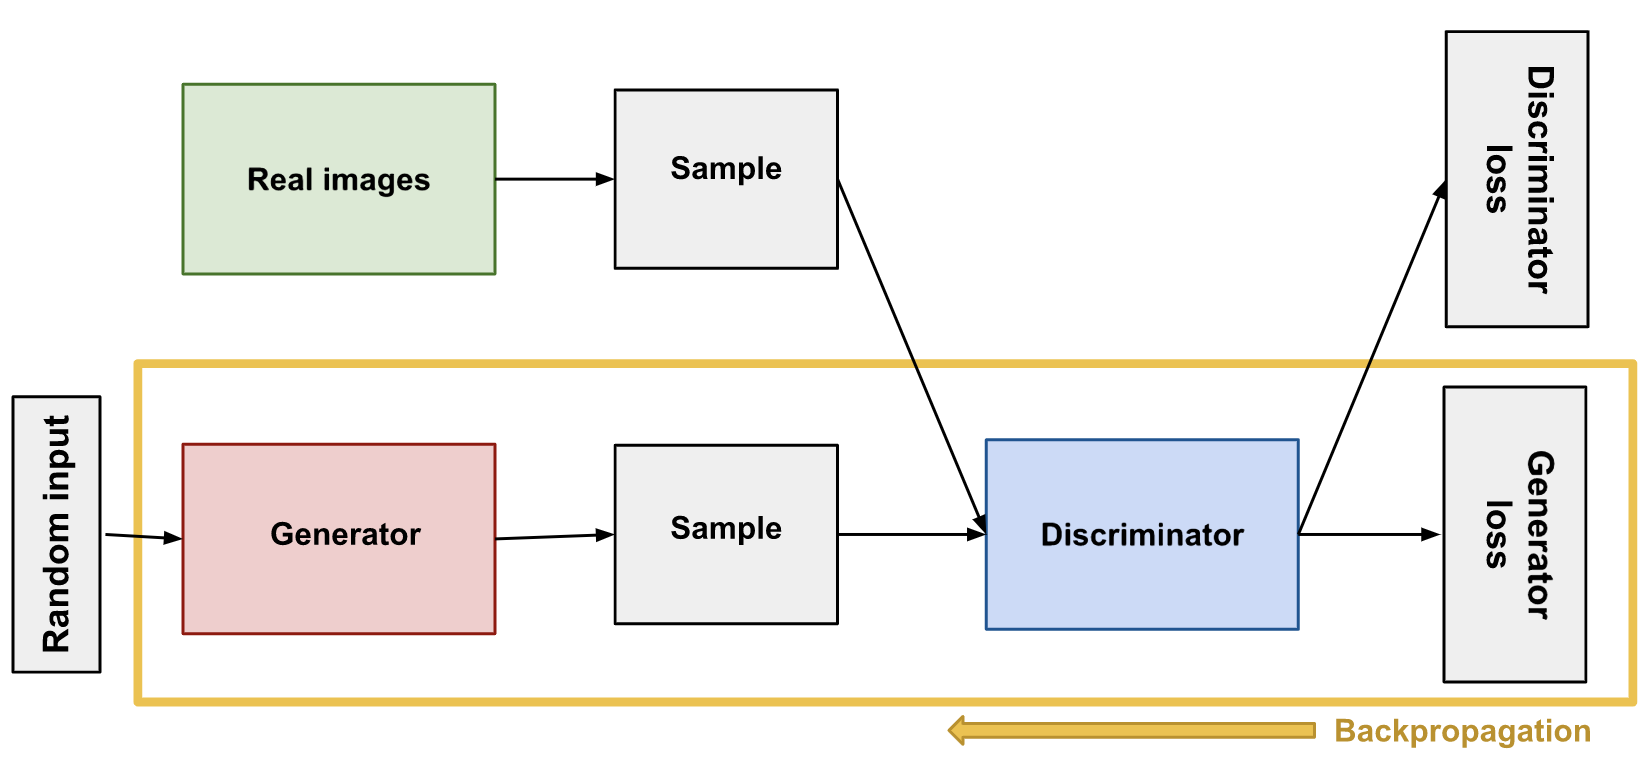
\includegraphics[width=1\textwidth]{fig/gan_architectur}
  \caption{GAN architecture
    \cite{google_bayesian_approach}.}
\end{figure}

After a brief introduction of GANs we focus now on the \textbf{Bayesian Approach}. One noteworthy work for data augmentation with the aid of the Bayesian model proposed by Toan Tran
et al. \cite{refrence_bayesian_approach}. In this approach, our deep learning model tries to estimate the
distributions of labeled data and uses the estimated distributions to optimize the latent
variable for data augmentation. The approach uses the GANs architecture skeleton to generate
synthetic data with the difference that the optimization of latent variables are derived from the Bayesian model.
The main idea for data augmentation using latent variables was proposed by the statistical learning
community \cite{Statistical_data_augmentation}. Nevertheless applying the idea directly into deep
learning seeks a massive computational effort. Therefore, the estimation of the variable
distribution becomes crucial. To be more precise, the
approach uses a novel Bayesian data augmentation algorithm, called Generalized Monte Carlo Expectation Maximization
(GMCEM). This algorithm augments training data and mutually optimizes the network parameters. The
algorithm successively generates synthetic data and uses the Monte Carlo Algorithm to estimate the expected value
of the network parameters given the previous estimate instead of calculating the loss function. After
the estimation of the expected value, the parameter values will be updated with stochastic gradient
descent (SGD). In the end, the algorithm and approach are turned in to reality with the aid of GANs. The
proposed GAN consists of one generator and two discriminators. As we discussed in Section
\ref{tit:Generative-Adversarial-Network} the generator is responsible to generate
synthetic data and one of our discriminators distinguishes fake and real data. However, the second
discriminator differentiates between the classes of data. Figure
\ref{fig:bayesian-approach-gan-architecture} represents the utilized network architecture in this
approach visually. This proposed architecture is almost similar to the Auxiliary Classifier GANs
(AC-GANS) \cite{AC_GANS}. Nevertheless, in the AC-GANS the discriminator is responsible for both
classifications real-or-fake data and data labels (classes) while in our network utilizes two
distinct discriminators for this matter.

\begin{figure}
  \centering
  \label{fig:bayesian-approach-gan-architecture}
  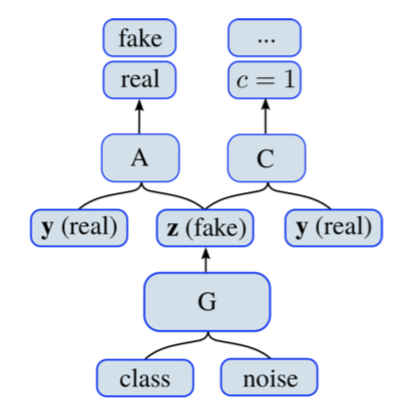
\includegraphics[width=0.5\textwidth]{fig/bayesian-approach-gan-architecture}
  \caption{The network architecture of Bayesian data augmentation approach \cite{refrence_bayesian_approach}. G: Generator, A: Authenticator, C: Classifier.}
\end{figure}

In the following, we will formally explain the utilized algorithm from the Toan Tran et al. work \cite{refrence_bayesian_approach}. The goal is to estimate the parameters of the neural networks using labeled data. The training process is defined by the following optimization problem:

\begin{equation} \label{eq:optimization-problem}
  \theta^{*}=\arg \max \log p(\theta | \mathbf{y}),
\end{equation}
where the training set is denoted as $\mathcal{Y}=\left\{\mathbf{y}_{n}\right\}_{n=1}^{N}$ with $y=(t,x)$
and $t\in\{1, ..., K\}$ (Classes-Set) and data samples $\mathbb{R}^D$ and $\theta$ are denoted as
model (network) parameters. The observed posterior defined as:
\begin{equation} \label{eq:observed-posterior}
  p(\theta | \mathbf{y})=p(\theta | t, \mathbf{x}) \propto p(t | \mathbf{x}, \theta) p(\mathbf{x} | \theta) p(\theta).
\end{equation}
Now if we assume that the data samples $\mathcal{Y}$ are conditionally independent, we can define the
following loss function which maximize the function given in (\ref{eq:optimization-problem}).

\begin{equation} \label{eq:loss-function}
  \log p(\theta | \mathbf{y}) \approx \log p(\theta)+\frac{1}{N} \sum_{l}^{N}\left(\log p\left(t_{n} | \mathbf{x}_{n}, \theta\right)+\log p\left(\mathbf{x}_{n} | \theta\right)\right)
\end{equation}
where $p(\theta)$ denotes a prior on the distribution of the deep learning model parameters, $p(t_n|x_n, \theta)$
represents the conditional likelihood of label $t_n$, and $p(x_n|\theta)$ is the likelihood of the
data $x$.

After estimation and optimization of $\theta$ on our training set, we generate
synthetic data from $y$ using the latent variable $z$. Therefore, the augmented $p(\theta | y,z)$ can be
estimated. The latent variable $z$, similar to $y$, is defined as $z = (t^{\alpha}, x^{\alpha})$ where
$t^{\alpha} \in \{1,...,K\}$ denotes the associated label and $x^{\alpha} \in   \mathbb{R}^D$ is a
synthesized sample. In order to avoid a heavy and most likely infinite computation we will use the Generalized Monte Carlo EM
Algorithm to estimate the expected value and maximize it instead of the Expectation-Maximization
(EM) algorithm. Hence the augmented posterior $p(\theta|y,
  z)$ for the latent variable $z$ is defined as follow:

\begin{equation} \label{eq:latent-variable}
  p(\theta | \mathbf{y}, \mathbf{z})=\frac{p(\mathbf{y}, \mathbf{z}, \theta)}{p(\mathbf{y}, \mathbf{z})}=\frac{p(\mathbf{z} | \mathbf{y}, \theta) p(\theta | \mathbf{y}) p(\mathbf{y})}{p(\mathbf{z} | \mathbf{y}) p(\mathbf{y})}=\frac{p(\mathbf{z} | \mathbf{y}, \theta) p(\theta | \mathbf{y})}{p(\mathbf{z} | \mathbf{y})}
\end{equation}
where the expectation step will be defined as:
\begin{equation} \label{eq:expectation-latent-variable}
  p(\theta | \mathbf{y}, \mathbf{z})=\frac{p(\mathbf{y}, \mathbf{z}, \theta)}{p(\mathbf{y}, \mathbf{z})}=\frac{p(\mathbf{z} | \mathbf{y}, \theta) p(\theta | \mathbf{y}) p(\mathbf{y})}{p(\mathbf{z} | \mathbf{y}) p(\mathbf{y})}=\frac{p(\mathbf{z} | \mathbf{y}, \theta) p(\theta | \mathbf{y})}{p(\mathbf{z} | \mathbf{y})}
\end{equation}
where \(\mathbf{z}_{m} \sim p\left(\mathbf{z} | \mathbf{y}, \theta^{i}\right),\) for \(m \in\{1,
\ldots, M\} .\) In \((6),\) if the label \(t_{m}^{a}\) of the \(m^{t h}\) synthesized sample
\(\mathbf{z}_{\mathbf{m}}\) is known, then \(\mathbf{x}_{m}^{a}\) can be sampled from the
distribution \(p\left(\mathbf{x}_{m}^{a} | \theta, \mathbf{y}, t_{m}^{a}\right) .\) Hence, the
conditional distribution \(p(\mathbf{z} | \mathbf{y}, \theta)\) can be decomposed as:

\begin{equation}
  p(\mathbf{z} | \mathbf{y}, \theta)=p\left(t^{a}, \mathbf{x}^{a} | \mathbf{y}, \theta\right)=p\left(t^{a} | \mathbf{x}^{a}, \mathbf{y}, \theta\right) p\left(\mathbf{x}^{a} | \mathbf{y}, \theta\right)
\end{equation}
where \(\left(t^{a}, \mathbf{x}^{a}\right)\) are conditionally independent of y given that all the
information from the training set y is summarized in \(\theta\). This means that \(p\left(t^{a} |
\mathbf{x}^{a}, \mathbf{y}, \theta\right)=p\left(t^{a} | \mathbf{x}^{a}, \theta\right),\) and
\(p\left(\mathbf{x}^{a} | \mathbf{y}, \theta\right)=p\left(\mathbf{x}^{a} | \theta\right)\).
Now, with respect to $\theta$ for the maximization step with concern of removing the independent terms
for $\theta$ will derive the maximization of $\hat{Q}\left(\theta, \theta^{i}\right)$ as follow:

\begin{equation}
  \begin{split}
    \hat{Q}(\theta, \theta^{i}) &= \log p(\theta)+\frac{1}{N} \sum_{n=1}^{N}(\log p(t_{n} | \mathbf{x}_{n}, \theta)+ \\
    & \log p(\mathbf{x}_{n} | \theta))+\frac{1}{M} \sum_{m=1}^{m} \log p(\mathbf{z}_{m} | \mathbf{y}, \theta) \\
    &= \\
    & \log p(\theta)+\frac{1}{N} \sum_{n=1}^{N}(\log p(t_{n} | \mathbf{x}_{n}, \theta)+\\
    & \log p(\mathbf{x}_{n} | \theta))+ \frac{1}{M} \sum_{m=1}^{n}(\log p(t_{m}^{a} | \mathbf{x}_{m}^{a}, \theta)+\log p(\mathbf{x}_{m}^{a} | \theta))
  \end{split}
\end{equation}

After all, we estimate the $\theta^{i +1}$ such that $\hat{Q}(\theta^{i +1}, \theta^{i}) >
  \hat{Q}(\theta^{i}, \theta^{i})$. To reduce the computation complexity, instead of using
gradient descent, we employ stochastic gradient decent (SGD) for estimating $\theta^{i +1}$. The
iteration will be continued until $|\theta^{i +1} - \theta^{i}|$ becomes sufficiently small.

The above formal explanations and equations are derived from \cite{refrence_bayesian_approach} and in some points are matched one-to-one.

%%%%%%%%%%%%%%%%%%%%%%%%%%%%%%
%%%%% Data Representation %%%%
%%%%%%%%%%%%%%%%%%%%%%%%%%%%%%
\chapter{Data Representation}
\label{tit:data-representation}
In this section, we briefly introduce the datasets that we use to evaluate the performance and
accuracy of each data
augmentation approach in practice. The reason behind our choice of datasets here is twofold. First,
they are well-known and widely used datasets. Many researchers already carried out numerous
experiments on them and reported results, and therefore a lot of baseline results are available for
the sake of comparison. Additionally, they are simple enough in their structure so that one can
relatively effortlessly learn and append non-complex classifiers, which can classify them with
desirable accuracy. The second reason is that all these datasets have ten classes with small
differences. They are balanced datasets which means each class consists of the same number of
samples. All of these help us to achieve a better and more realistic benchmark.

\section{MNIST}
The MNIST dataset (Modified National Institute of Standards and Technology) is a large handwritten
digits dataset, provided by Yann Le Cun, derived from NITS Special Database 19 \cite{NIST}.

The MNIST dataset consists of $60,000$ train- and $10,000$ test-images where each image is grayscale
with $28 \times 28$ pixels. The dataset has ten classes where each class represents a digit from
zero to nine. The data is fairly
splitted between classes \cite{MNIST_data_reference}. The MNIST is one of the most popular datasets for
deep learning because of its low complexity and compatibility with almost all deep learning
models. Hence, many papers attempted to reach a low error-rate on this dataset. One of them manages
to reduce the error-rate on the MNIST by up to $0.23\%$ \cite{MNIST_best_result_reference}. You can
find the information about the dataset in Table
\ref{dataset_table}. Figure \ref{fig:mnist_dataset_example} shows an example of the dataset.

\begin{figure}
  \centering
  \label{fig:mnist_dataset_example}
  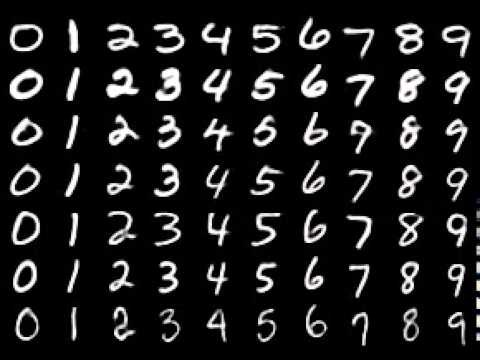
\includegraphics[width=0.5\textwidth]{fig/mnist}
  \caption{7 examples per class of MNIST dataset, merged in one image \cite{MNIST_dataset_example}.}
\end{figure}


\section{Fashion-MNIST}
Fashion-MNIST is a dataset of Zalando's\footnote{\url{https://jobs.zalando.com/de/tech/}}
article images provided by Han Xiao et al. \cite{Fashion_MNIST_reference} for benchmarking machine learning algorithms.

Pretty much similar to the MNIST dataset, the Fashion-MNIST dataset, consists of $60,000$ train- and
$10,000$ test-images where each image is grayscale
with $28 \times 28$ pixels. It has ten classes (T-Shirt, Trouser, Pullover, Dress, Coat,
Sandal, Shirt, Sneaker, Bag, Ankle Boot) and the data is fairly
split between these classes. One of the best reported accuracy achieved $91.90\%$ on this dataset
with a convolutional neural
network\footnote{\url{https://github.com/zalandoresearch/fashion-mnist\#benchmark/}}. You can
find the information about the dataset in Table
\ref{dataset_table}. Figure \ref{fig:fashion_mnist_dataset_example} shows an example of the dataset.


\begin{figure}
  \centering
  \label{fig:fashion_mnist_dataset_example}
  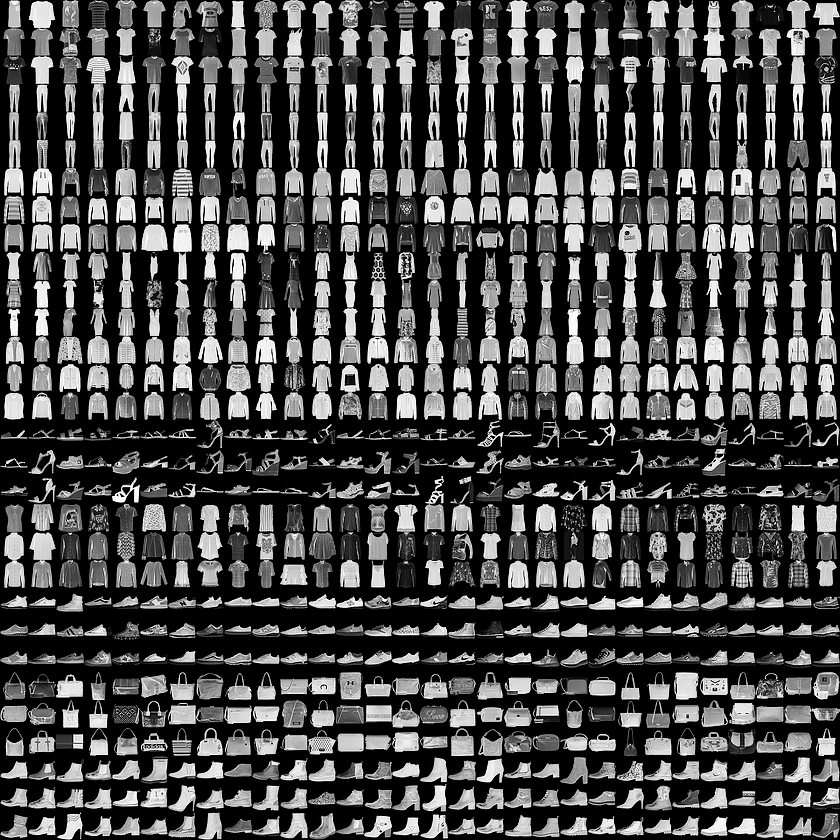
\includegraphics[width=0.5\textwidth]{fig/fashion-mnist-dataset_example}
  \caption{Examples of Fashion-MNIST dataset, merged in one image.}
\end{figure}

\section{CIFAR-10}
The CIFAR-10 (Canadian Institute for Advanced Research)
, collected by Alex Krizhevsky, Vinod Nair, and Geoffrey Hinton is a subset of $80$ million tiny
images dataset \cite{CIFAR-10_origin_dataset}.

The dataset consists of $60,000$  RGB with $32 \times 32$ pixels images, which are divided into $50,000$ train and $10,000$ test datasets. As the name makes it clear, the CIFAR-10 contains ten classes (plane, car, bird, cat, deer, dog, frog, horse, ship, truck) \cite{CIFAR-10_dataset_reference}.
One of the lowest reported error-rates achieved $2.56\%$ with a convolutional neural network \cite{CIFAR-10_best_result_reference}. You can
find the information about the dataset in Table
\ref{dataset_table}. Figure \ref{fig:cifar-10_dataset_example} shows an example of the dataset.

\begin{figure}
  \centering
  \label{fig:cifar-10_dataset_example}
  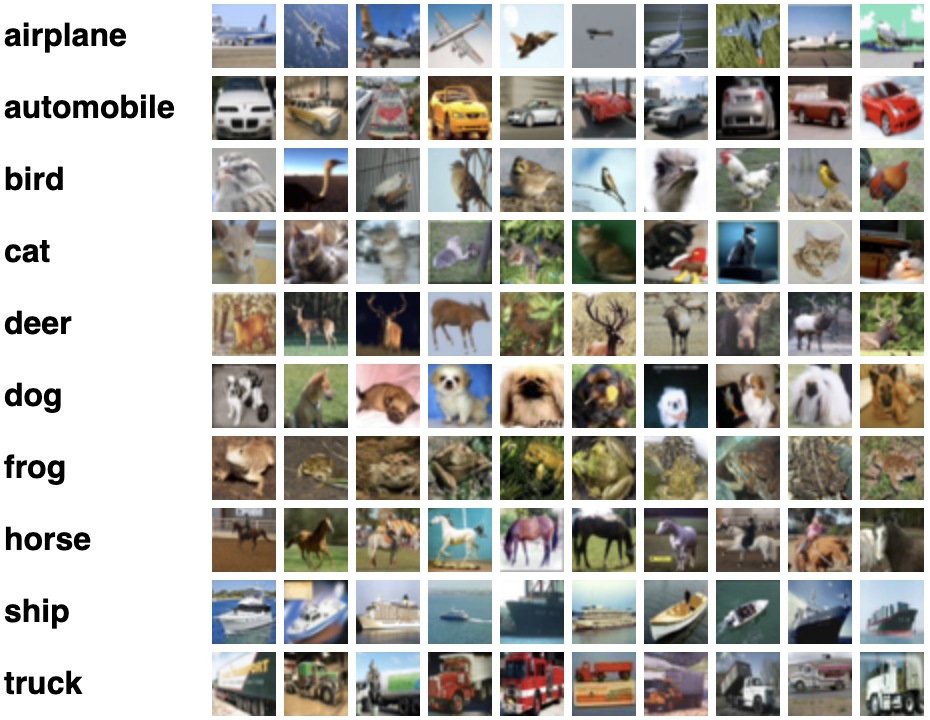
\includegraphics[width=0.5\textwidth]{fig/cifar-10}
  \caption{10 examples per class of CIFAR-10 dataset, merged in one image \cite{CIFAR-10_dataset_reference}.}
\end{figure}




\begin{table}[]
  \label{dataset_table}
  \begin{tabular}{
      l |
      c
      c
      c
      c
      c}
    \hline
    {\textbf{Dataset}}       & \multicolumn{1}{l}{{\textbf{NO. Classes}}} & \multicolumn{1}{l}{{\textbf{NO. Train}}} & \multicolumn{1}{r}{{\textbf{NO. Test}}} & \multicolumn{1}{l}{{\textbf{Size (pixel)}}} & \multicolumn{1}{l}{{\textbf{NO. Channel}}} \\ \hline
    {\textbf{MNIST}}         & 10                                         & 60,000
                             & 10,000                                     & $28\times28$                             & 1
    (Grayscale)                                                                                                                                                                                                                                           \\
    {\textbf{Fashion-MNIST}} & 10                                         & 60,000
                             & 10,000                                     & $28\times28$
                             & 1 (Grayscale)                                                                                                                                                                                                              \\
    {\textbf{CIFAR-10}}      & 10                                         & 50,000
                             & 10,000                                     & $32\times32$                             & 3
    (RGB)                                                                                                                                                                                                                                                 \\ \hline
  \end{tabular}
  \caption{Structure of datasets.}
\end{table}


\chapter{Experiments}
In this chapter, we explain the manner of implementation of the classifiers, approaches, and
techniques pragmatically. We introduce the architecture of the utilized
classifiers\footnote{Convolutional Neural Networks (CNNs)} for each introduced dataset in Chapter
\ref{tit:data-representation}. After that, we explain the procedure of implementation of each
introduced approach and technique in Chapter \ref{tit:data-augmentation}.

\section{CNNs Architecture}
In this section, we will introduce our classifiers' architecture. We picked our CNNs architecture from
different sources regarding their low complexity and desirable accuracy.  It might be that our chosen
CNNs architecture does not provide the best-reported accuracy on dataset. However, as we use the
same CNN-architecture for each dataset and we aim to compare various data augmentation approaches on
each dataset, it would not affect our results.
%Moreover, as we will report in chapter (\ref{tit:results})
%our result are not so far away from best-reported accuracy on the original dataset.

\subsection{MNIST}
For the MNIST dataset, we have chosen a semi-simple CNN architecture from
\cite{MNIST_CNN_Architecture} with two
convolutional layers and two fully connected layers. ReLU function is utilized as the activation
function. For training and to calculate the loss function, \textbf{CrossEntropyLoss} and
to optimize the network's parameters \textbf{Adam optimizer} \cite{adam_optimizer} from the Pytorch have been
chosen. The learning rate for Adam optimizer is set to $0.001$. To reduce overfitting, a
drop-out layer is placed at the end of the second convolutional layer. Figure \ref{fig:MNIST_CNN_Architecture} represents the explained CNN architecture visually.

\begin{figure}
  \centering
  \label{fig:MNIST_CNN_Architecture}
  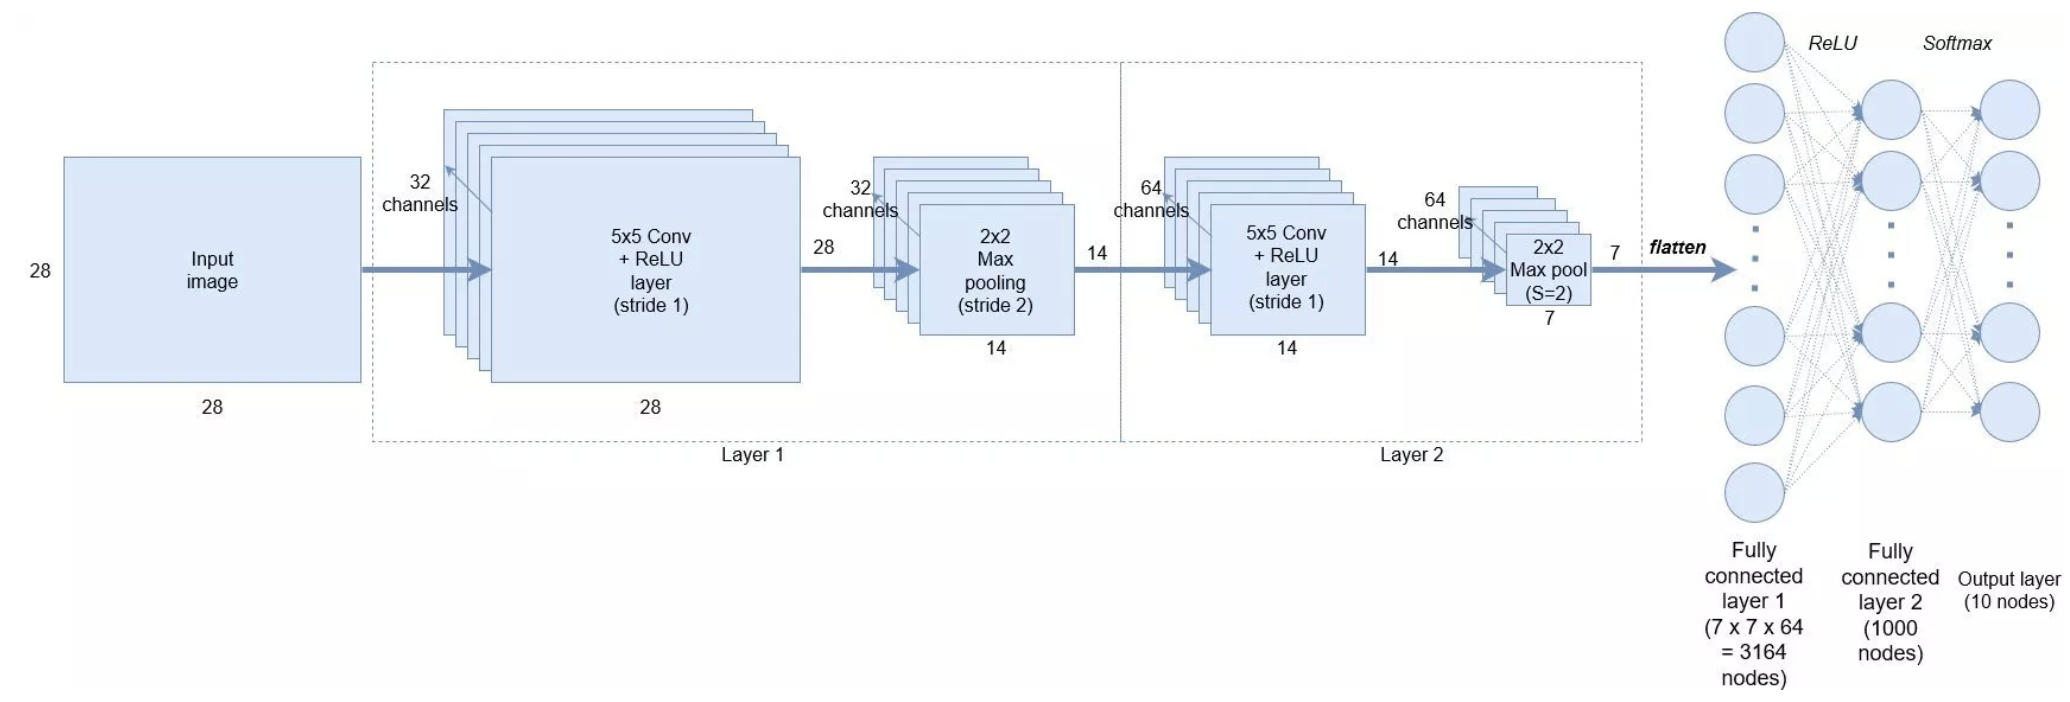
\includegraphics[width=1\textwidth]{fig/MNIST-CNN-Architecture}
  \caption{CNN Architecture for training the MNIST dataset \cite{MNIST_CNN_Architecture_Image}.}
\end{figure}


\subsection{Fashion-MNIST}
The Fashion-MNIST dataset uses CNN architecture derived from \cite{FashionMNIST_dataset_example} with two
convolutional layers and two fully connected layers similar to the MNIST dataset but with
different of up- and downsampling and kernel sizes. ReLU function is utilized as the activation
function. The learning rate for Adam optimizer is set to $0.001$. Figure \ref{fig:Fashion_MNIST_CNN_Architecture} represents the explained CNN architecture visually.

\begin{figure}
  \centering
  \label{fig:Fashion_MNIST_CNN_Architecture}
  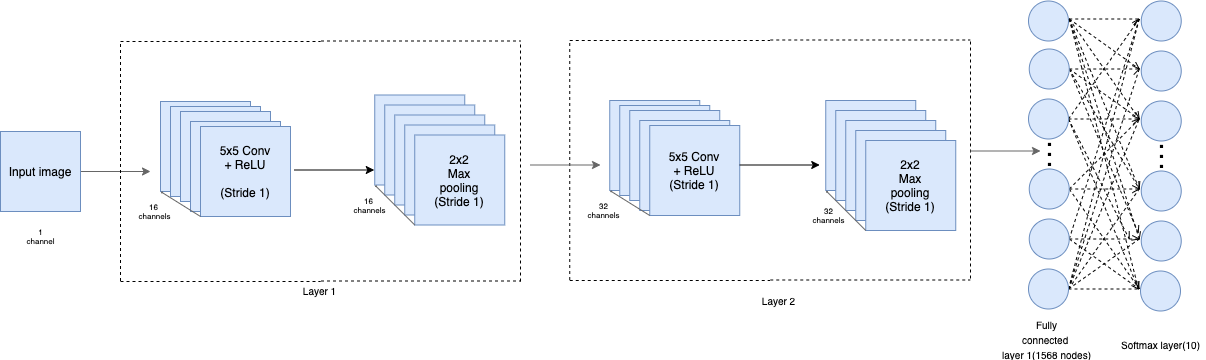
\includegraphics[width=1\textwidth]{fig/Fashion-MNIST-CNN-Architecture}
  \caption{CNN Architecture for training the Fashion-MNIST dataset.}
\end{figure}

\subsection{CIFAR-10}
For the CIFAR-10 dataset, we have chosen a bit more complex CNN architecture from
\cite{CIFAR_CNN_Architecture} with six
convolutional layers and three fully connected layers. ReLU function is utilized as the activation
function. For training and to calculate the loss function, \textbf{CrossEntropyLoss} and
to optimize the network's parameters \textbf{Adam optimizer} similar to the two previous CNNs architectures have been
chosen. The learning rate for Adam optimizer is set to $0.001$. To reduce overfitting, a
drop-out layer is placed at the end of the fourth convolutional layer. Figure \ref{fig:CIFAR_CNN_Architecture} represents the explained CNN architecture visually.


\begin{figure}
  \centering
  \label{fig:CIFAR_CNN_Architecture}
  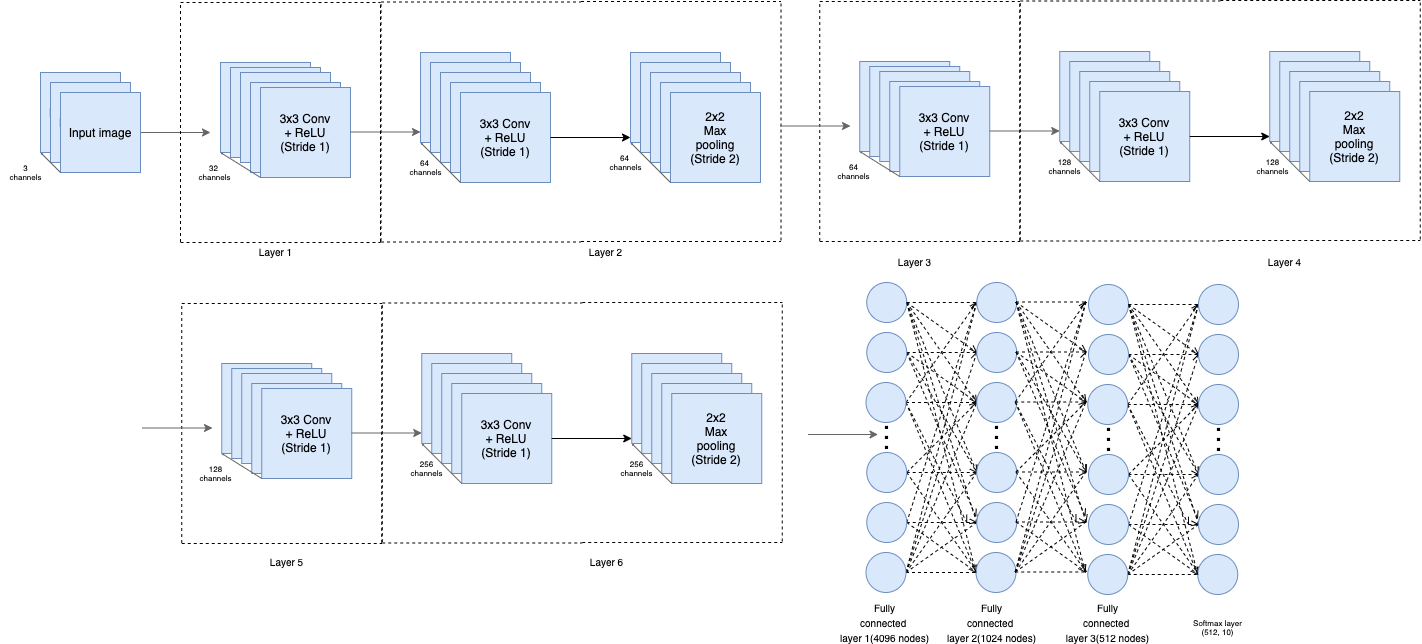
\includegraphics[width=1\textwidth]{fig/CIFAR-CNN-Architecture}
  \caption{CNN Architecture for training the CIFAR-10 dataset.}
\end{figure}

\section{Implementations}
In what follows, we will briefly explain the manner of implementation of each
approach and technique.

In order to put the idea of label preserving transformations and their techniques
into practice, we utilized an external library in Python for data augmentation called
Augmentor\footnote{\url{https://github.com/mdbloice/Augmentor}}. The main part (Learning) is carried
out by a powerful library by Facebook called Pytorch\footnote{\url{https://pytorch.org/}}.

\subsection{Image Translations}
To augment the data with image translation we picked patches smaller than original image size with
a factor of approximately $0.8$. The patches are not only wide enough to not lose the $80\%$ of the image but
also allow to augment the dataset with factor close to $100$. The equation
(\ref{eq:reproduce_image_translate_size}) reproduces equation (\ref{eq:image_translate}) with
the MNIST dataset. After augmentation with translations and their horizontal reflections, we resized images with bilinear interpolation to the original image size in the dataset. This matter provides this possibility to be able to change the patches' size without putting any afford to modify CNN architecture.

\begin{equation}
  \label{eq:reproduce_image_translate_size}
  2\times(28-(28 \times 0.8)+1)\times(28-(28 \times 0.8)+1) \approx 2 \times 7 \times 7 \approx 100
\end{equation}

For test and prediction, the image augmented with the same size of patches from corners and center
with a factor of ten.

\subsection{Elastic Distortions}
To augment with this technique we picked $100$ different and random patches from the image with a
size of $8 \times 8$ and displacement performed in these patches with $\alpha = 8$ to augment the
data with factor $100$.  After displacement, the patches have been smoothed with the Gaussian filter
with $\sigma = 4$. For test and prediction, we used the same parameters but this time augmented with
a factor of ten instead of $100$.

\subsection{Stroke Warping}
For stroke warping, we augmented each image with skewing them horizontally and vertically with
different magnitude, rotated them clockwise and counterclockwise with $-10^{\circ} \leq \alpha \leq
  10^{\circ}$, and scaled with a factor s where $-6 \leq s \leq 6$  and sheared them. With different
values for the mentioned parameters, we augmented the data with a factor of $100$. Similar to other
for test and prediction data augmented with a factor of ten.

\subsection{Bayesian Approach}
Here we used the same code\footnote{https://github.com/toantm/pytorch-bda}, implemented by Toan Tran et
al. and introduced in their work \cite{refrence_bayesian_approach} with small modification for using
it on few-shot dataset.


\chapter{Result \& Comparison}
\label{tit:results}
In this Chapter, first, we give the main results of our experiments using introduced approaches as
well as introduced datasets. Following the main findings is a discussion of the advantages and
drawbacks of each method and a comparison of its behaviour on different datasets. Besides providing
great insights, this discussion serves as a preface and sets the stage for the novel ideas and
approaches proposed in the next chapter.

\section{Result}
For the sake of an insightful and comprehensive comparison, we implement each technique or approach
using different setups. Precisely speaking, we consider the accuracy of each method using the
original dataset, that is, including all the test and train data points, as well as the accuracy
using few-shot datasets both with and without augmentation. Our results also consist of a comparison
between various $k$-shot\footnote{$k$ represents the number of samples in training set, existing in
  each class.} datasets:

\begin{equation}
  k=
  \begin{cases}
    \{1, 5, 10\}   & \text{if}\ dataset=
    \ MNIST \ or \ Fashion-MNIST                    \\
    \{10, 20, 30\} & \text{if}\ dataset= \ CIFAR-10
  \end{cases}
\end{equation}

Additionally, to compare the result in fair circumstances we augmented the data by a factor of 100 (100X)
for the training and by a factor of ten (10X) with each augmentation technique. To provide
a more realistic result, we used 10-fold cross-validation \cite{cross_validation}. That means for each k-shot learning, we
derived ten different and random k-shot datasets to calculate more realistic accuracy for each
technique.

Figures \ref{fig:MNIST_result}, \ref{fig:Fashion_MNIST_result}, and
\ref{fig:CIFAR_10_result} represent the results and accuracy for
MNIST, Fashion-MNIST, and CIFAR-10 datasets, respectively.


\begin{figure}
  \centering
  \label{fig:MNIST_result}
  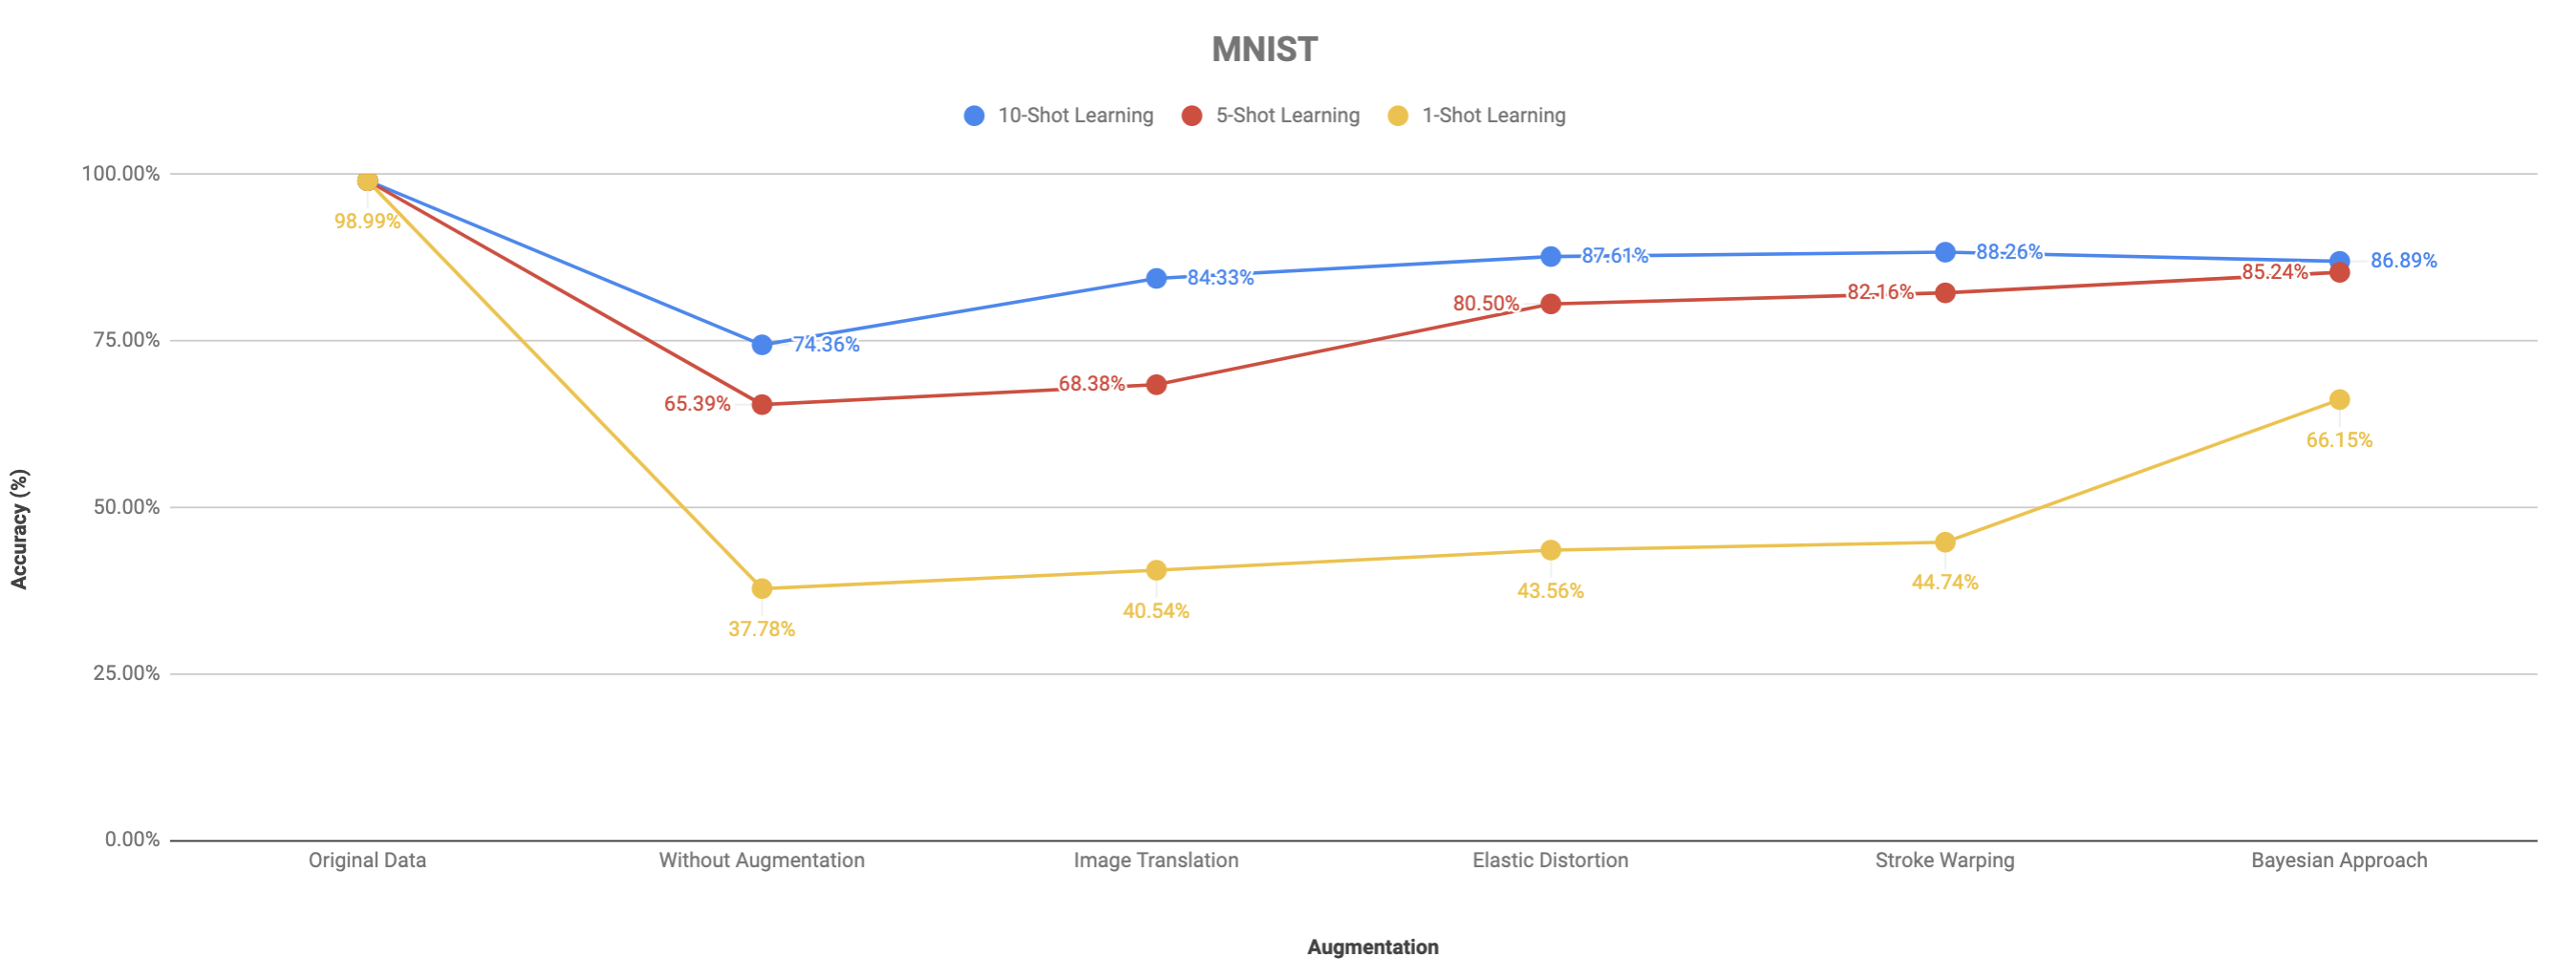
\includegraphics[width=1\textwidth]{fig/result/mnist-result}
  \caption{Result of augmentation techniques on MNIST dataset.}
\end{figure}


\begin{figure}
  \centering
  \label{fig:Fashion_MNIST_result}
  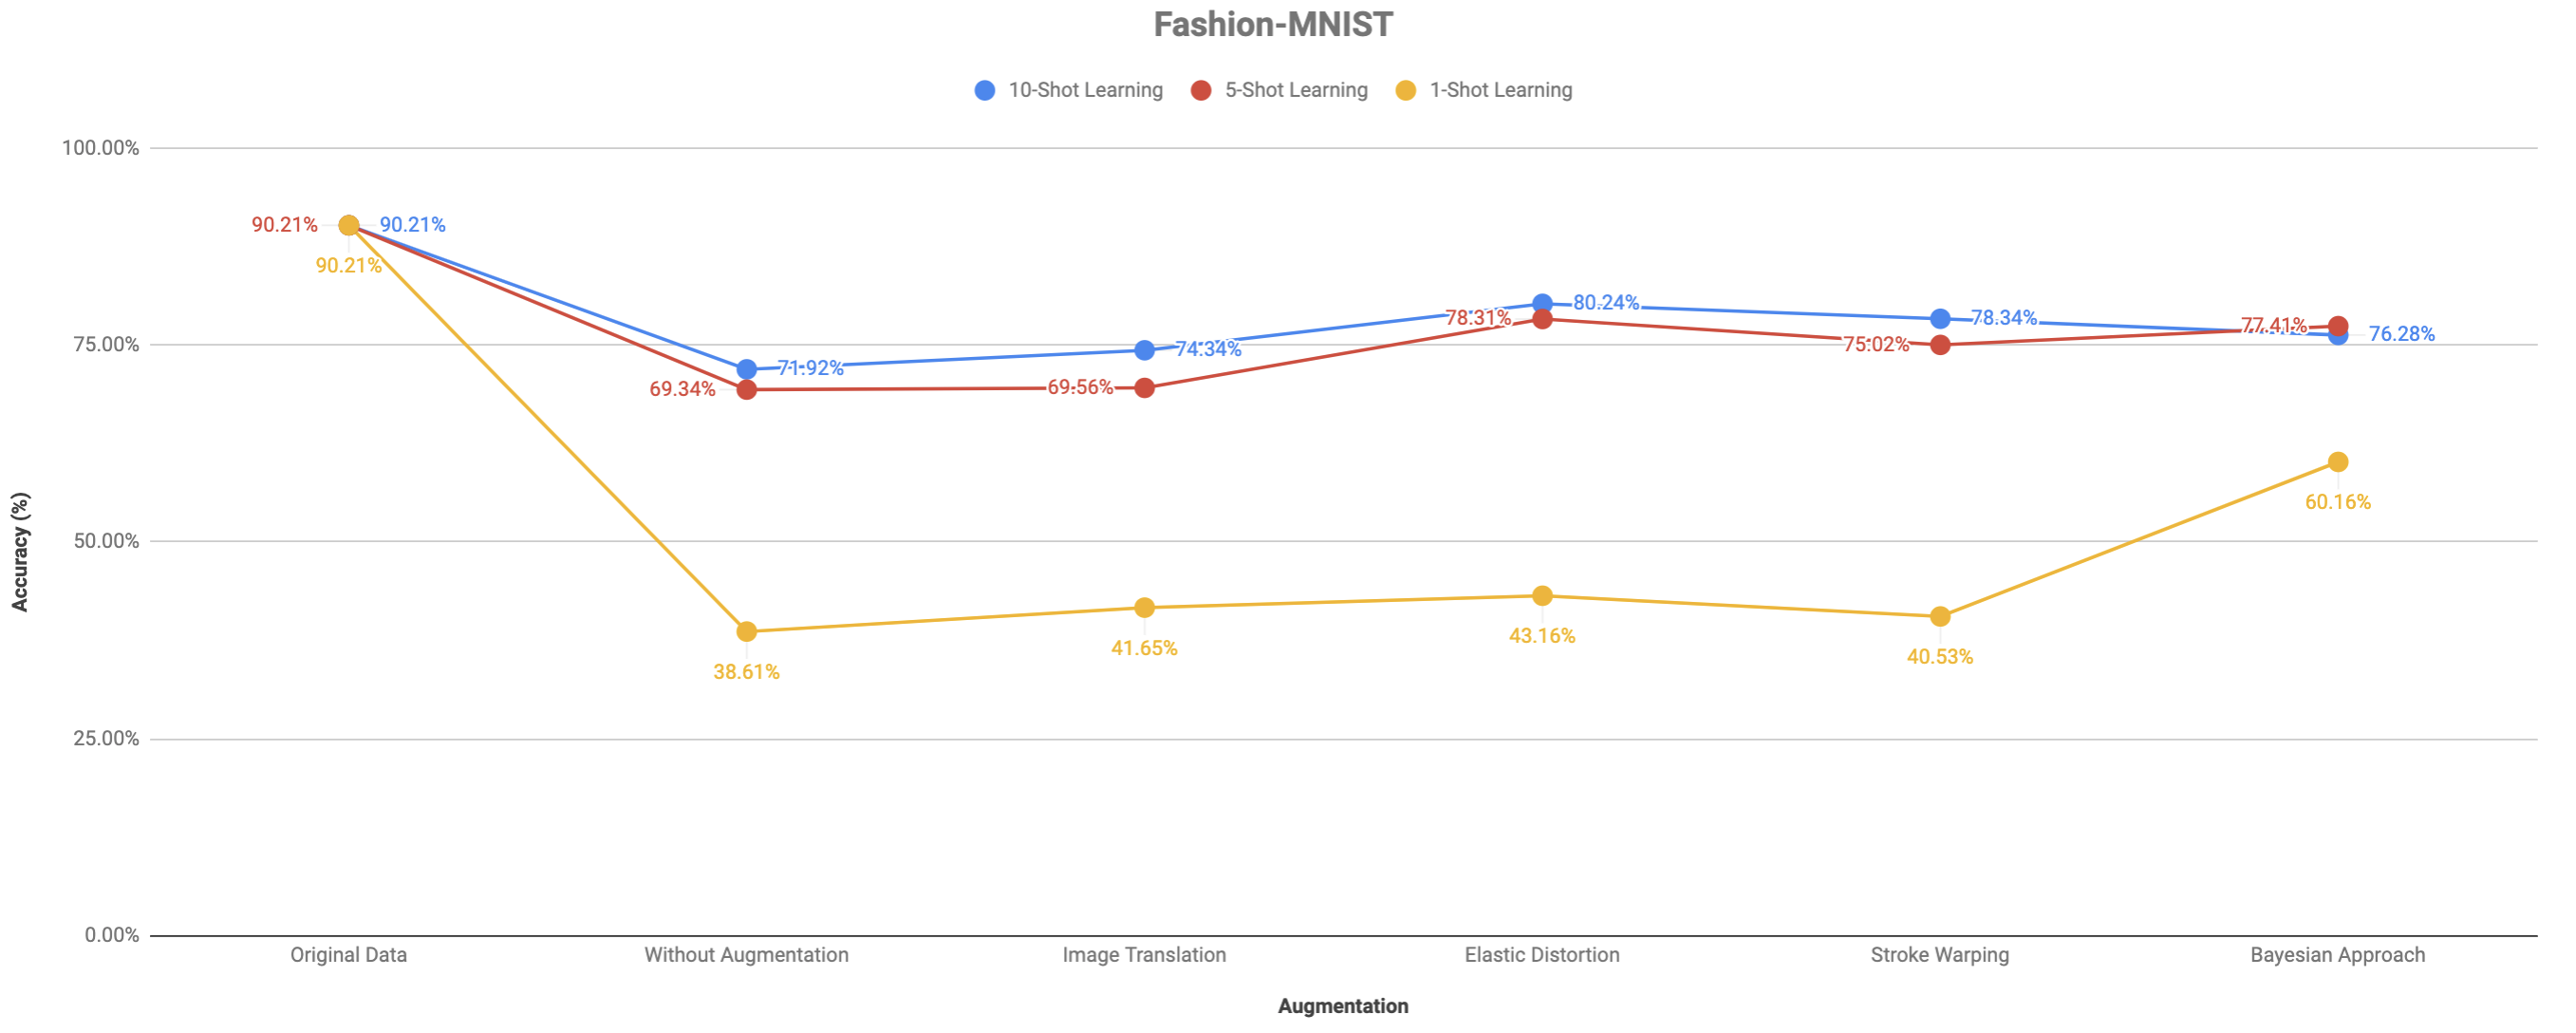
\includegraphics[width=1\textwidth]{fig/result/fashion-mnist-result}
  \caption{Result of augmentation techniques on Fashion-MNIST dataset.}
\end{figure}


\begin{figure}
  \centering
  \label{fig:CIFAR_10_result}
  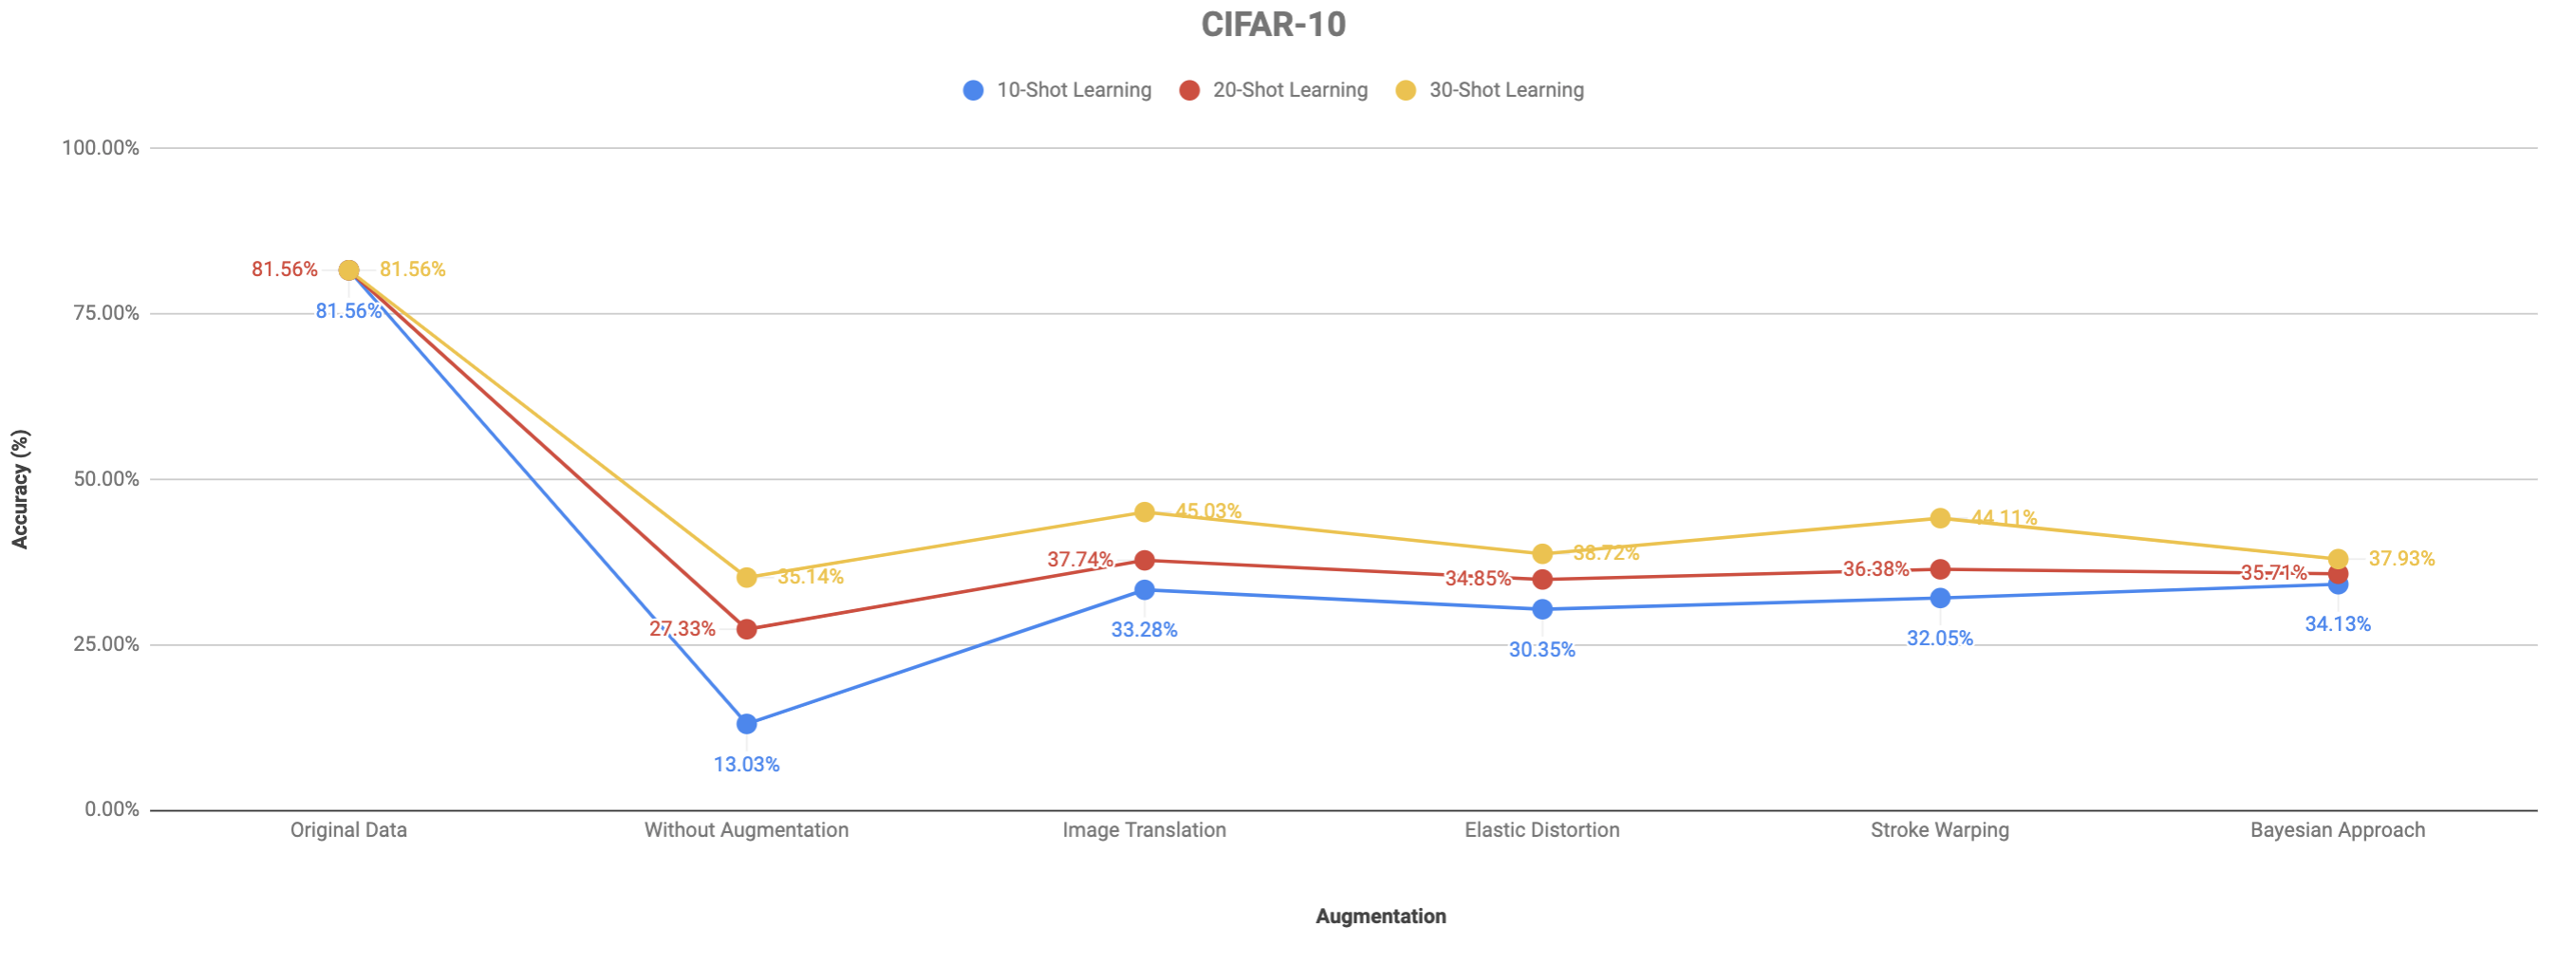
\includegraphics[width=1\textwidth]{fig/result/cifar-10-result}
  \caption{Result of augmentation techniques on CIFAR-10 dataset.}
\end{figure}

The first look at Figures \ref{fig:MNIST_result} and \ref{fig:Fashion_MNIST_result} expose that there is
a significant gap between the accuracy of 10 and 5-shot learning and 1-shot learning without augmentation. Besides,
it shows that k-shot learning is not linearly correlated with the accuracy for each technique. As there is
just one sample for each class, the CNN involves pretty soon with overfitting. Nevertheless, the
accuracy is about $30\%$ and that means that the prediction is not random even for 1-shot
learning on MNIST and Fashion-MNIST.

Figure \ref{fig:CIFAR_10_result} displays the considerable gap
between accuracy on the original data and few-shot learning on CIFAR-10. This matter exposes the major
role of color (RGB images) in learning and accuracy. As it expected, this gap is not observable on MNIST
and Fashion-MNIST.

\section{Comparison}

Table \ref{tb:result_table}, derived from the Figures \ref{fig:MNIST_result}, \ref{fig:Fashion_MNIST_result}, and
\ref{fig:CIFAR_10_result} for 10-shot datasets, determines that the augmentation approaches and
techniques behave similar on MNIST and Fashion-MNIST datasets. That means the improvement rate of
accuracy is almost the same for all techniques. On the other hand, some techniques behave
differently on CIFAR-10 in comparison to MNIST and Fashion-MNIST datasets. In what follows, we will
discuss each technique behavior on the datasets and the underlying reasons.

\begin{table}[]
  \label{tb:result_table}
  \resizebox{\textwidth}{!}{%
    \begin{tabular}{l|ccccc}
      \hline
      \textbf{Dataset\textbackslash{}Augmentation} & \multicolumn{1}{l}{\textbf{Without Augmentation}} & \multicolumn{1}{l}{\textbf{Image Translations}} & \multicolumn{1}{l}{\textbf{Elastic Distortions}} & \multicolumn{1}{l}{\textbf{Stroke Warping}} & \multicolumn{1}{l}{\textbf{Bayesian Approach}} \\ \hline
      \textbf{MNIST}                               & $74.36\%$                                         & $84.33\%$                                       & $88.26\%$                                        & $87.61\%$                                   & $86.89\%$                                      \\
      \textbf{Fashion-MNIST}                       & $71.92\%$                                         & $74.34\%$                                       & $80.24\%$                                        & $78.34\%$                                   & $76.28\%$                                      \\
      \textbf{CIFAR-10}                            & $13.03\%$                                         & $33.28\%$                                       & $30.35\%$                                        & $32.05\%$                                   & $34.13\%$                                      \\ \hline
    \end{tabular}%
  }
  \caption{Accuracy of augmentation techniques on 10-shot datasets.}
\end{table}

\subsection{Image Translations}
As Table \ref{tb:result_table} represents firmly, image translation has the best accuracy on CIFAR-10 as it
was expected. On the other hand, the accuracy of MNIST and Fashion-MNIST for image translation is not
as good as the other techniques. It has the worse performance on these datasets. The reason is
that image translation works with image patches smaller than the original image size. Hence, its
performance is highly dependent on the datasets and even their classes. Put the matter in another
way, image translation sometimes extracts patches from an image of class but the generated synthetic
image gets the same as an image in another class. For example, Figure \ref{fig:image_translation_example_bad_accuracy} shows a translation of
digit nine from the MNIST dataset which looks like a zero. On the Fashion-MNIST dataset some patches
of a shirt image can become similar to a T-shirt image, etc. but the image translation on the CIFAR-10
dataset does not map the synthetic images to another class. It means a patch of e.g. an airplane will
not become similar to another class in the CIFAR-10 dataset.
\begin{figure}
  \centering
  \label{fig:image_translation_example_bad_accuracy}
  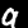
\includegraphics[width=0.5\textwidth]{fig/result/Image_translations_mnist}
  \caption{Example of Image Translations on digit $9$ which looks like $0$.}
\end{figure}

\subsection{Elastic Distortions}
As represented in Table \ref{tb:result_table}, elastic distortion has the best performance on
MNIST and Fashion-MNIST. This behavior is what we expected from elastic distortion regarding its
augmentation technique. For example, on the MNIST dataset, it simulates the deformation and flexion
caused by handwriting on the digits and generates the synthetic data almost like the real ones in
the original dataset. Figure \ref{fig:Elastic_Distortion_Example} represents this matter visually.
Fashion-MNIST obeys the same reason. In this case, the distortions simulate for example the folding
on clothes and generate the synthetic data almost like the real other ones in the original dataset.
On the other hand, the accuracy of elastic distortion on CIFAR-10 is not as good as the other
techniques and the reason is trivial as well. Distortions, for example on cars or airplanes will not
generate a total new meaningful image that are close to the other ones in the original
dataset.

\begin{figure}
  \centering
  \label{fig:Elastic_Distortion_Example}
  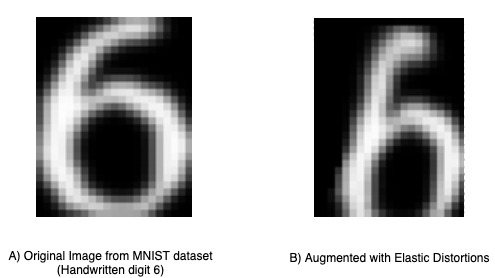
\includegraphics[width=1\textwidth]{fig/result/Elastic-Distortions-Example}
  \caption{Example of Elastic Distortions on one of the MNIST data.}
\end{figure}

\subsection{Stroke Warping}
Table \ref{tb:result_table} demonstrates that stroke warping is the most robust technique between
the other mentioned techniques in the label preserving transformation approach. It means the
accuracy improvement is almost the same for all three datasets. The reason is that Stroke Warping
makes small changes in the whole image and only partially. These small changes help to improve the
accuracy however the performance and accuracy of this technique is always ordinary on all datasets in compare to the
other techniques.


\subsection{Bayesian Approach}
Table \ref{tb:result_table} shows that the bayesian approach is
another robust approach and class of technique on different datasets. Since we learn during the
augmentation how to generate the synthetic data and unlikely of the label preserving transformations
the data will not be generated with some pre-defined transformations, this approach improves the
accuracy with a factor independent to the dataset. However, this approach improves the accuracy
relatively well and is robust on different datasets. In comparison to the other techniques requires
a long time during generating and training phase. Additionally, since this approach works with
statistical models and distributions (Max-A-Posterior probability, the accuracy stays almost constant in
1-shot learning. On the another hand, if the number of samples is increased, the accuracy
increases more, compare to other techniques.

\section{Conclusion}
Between label preserving transformation techniques, image translation, and elastic distortion are
highly dependent on datasets and even classes which means they can provide a desirable accuracy on
some classes and some classes are not suitable for such an augmentation. This matter makes them
strong with a considerable improvement in accuracy on compatible datasets and not so strong on
incompatible ones. This is based on the number of suitable classes for such an augmentation.

Stroke warping is the most robust technique of label preserving transformations which means they improve the accuracy with almost the same factor independent on datasets. This technique is suitable for almost all datasets but the improvement of accuracy is always less than the best case of image translation and elastic distortion.

Bayesian approach is another class of techniques which provides robust result and accuracy on all
datasets. The advantage is that it learns how to augment the data and generate the synthetic data
based on each dataset and obtainable samples. On the another hand, high time-complexity in comparison
with other techniques is a disadvantage of this kind of augmentation. Additionally, as it works with
statistical models and distributions the number of samples at the beginning playing a significant
role in the final result.

\chapter{Contribution Of Work}
\label{tit:Contribution_of_Work}
In this chapter, we will introduce three new techniques of data augmentation, developed in this
work. We studied some of the existing techniques and experimented pragmatically on three different
datasets and compared them comprehensively in previous chapters. Based on all these studies and the
aid and inspiration of other existing works and researches, we aim to propose new techniques for
data augmentation to rectify the disadvantage of existing ones to reach better results and accuracy.
In what follows, we focus on each approach (label preserving transformations and bayesian approach)
separately and propose an improvement for each approach and their techniques.

\section{Ensemble Learning \& Label Preserving Transformations}
As we precisely cleared in the previous Chapter \ref{tit:results} label preserving
transformations techniques are highly dependent on datasets or even on each class (at least image
translation and elastic distortion). This matter makes them perform completely different on
datasets in each class. Put the matter in another way, they can have highly
good accuracy and prediction in one class, while having extremely low accuracy and prediction in another
class from the same dataset. Figure \ref{fig:Fashion_MNIST_Heatmaps} represents an example of this
matter of the predicted class
and the actual class of the 10-shot learning on the Fashion-MNIST dataset for different label
preserving transformation techniques.

\begin{figure}
  \centering
  \label{fig:Fashion_MNIST_Heatmaps}
  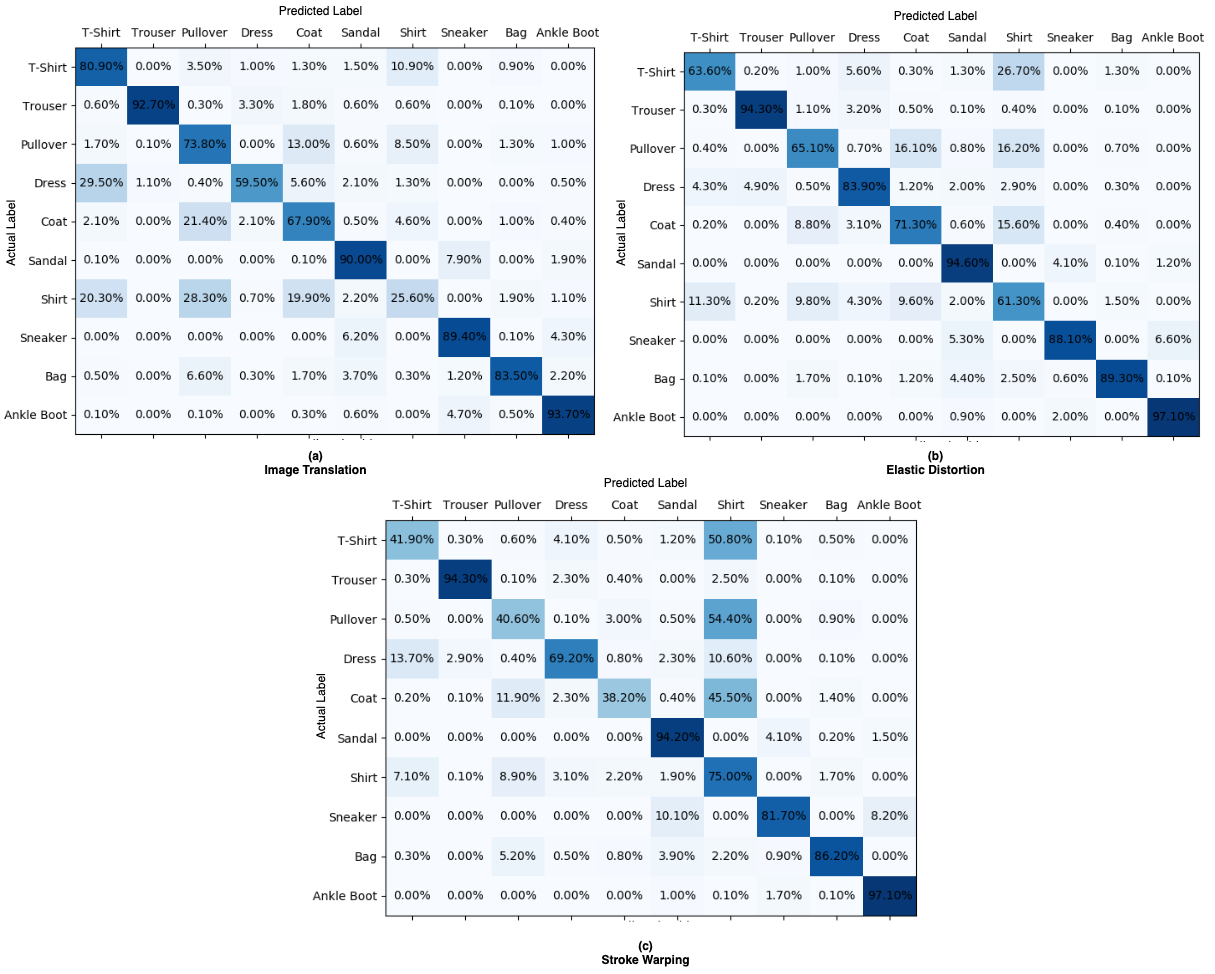
\includegraphics[width=1.1\textwidth]{fig/contribution/Fashion_MNIST_Heatmap}
  \caption{Prediction accuracy of each class on Fashion-MNIST for Label Preserving Transformations techniques.}
\end{figure}

As the astute readers most likely can guess in this technique we will propose a combination of image
translation, elastic distortion, and stroke warping. However, the combination will be accompanied
by learning from the performance of each technique in each class and try to choose the best
technique for each class. In this technique and for such learning we were inspired by a well-know
approach called Ensemble Learning introduced by Robi Polikar \cite{ensemble_learning}. This technique begins with the
augmentation and learning for each three label preserving transformations techniques (image
translation, elastic distortion, and stroke warping) separately. After training and with testing
dataset a heatmap ($10 \times 10$ prediction matrix) for accuracy on each class will be generated
for each technique as shown in Figure \ref{fig:Fashion_MNIST_Heatmaps}. These matrices expose the
performance and accuracy of each augmentation technique for each class. Based on these matrices, a
matrix will be generated which represents the probability of correct prediction for each class with
each augmentation technique. In the end, we augment again our few-shot dataset, but this time with
the highest correct prediction probability technique for each class and train the CNN with this
augmented dataset. This is how we augment each class with the best techniques and improve the whole
accuracy on each dataset. The following equation shows the manner of generation of correct prediction probability formally:

Let IT, ED, and SW be the $10 \times 10$ prediction matrices for image translation,
elastic distortion, and stroke warping respectively and each element of them is denoted by $it_{ij}$, $ed_{ij}$,
and $sw_{ij}$ respectively for $i,j \in \{1,2,...,10\}$ and $i=j$, then the correct prediction probability
matrix denoted by CPP and each element by $cpp_{kj}$ will be generated as follow:
\begin{equation}
  \begin{aligned}
    cpp_{kj} =
    \begin{cases}
      \dfrac{it_{ij}}{it_{ij} + ed_{ij} + sw_{ij}} & \text{if}\ k=1 \\ \\
      \dfrac{ed_{ij}}{it_{ij} + ed_{ij} + sw_{ij}} & \text{if}\ k=2 \\ \\
      \dfrac{sw_{ij}}{it_{ij} + ed_{ij} + sw_{ij}} & \text{if}\ k=3
    \end{cases}
  \end{aligned}
\end{equation}

Where $j \in \{1,2,...,10\}$, then the augmentation technique for each class will be determined by:
\begin{equation}
  \begin{aligned}
    Augmentation \ Technique_{j} = max(cpp_{kj}) \ \ \ \ , \ \forall k \in \{1,2,3\}
  \end{aligned}
\end{equation}

At the end and in the test and prediction time, we augment the data by a factor of ten with all three
techniques. Again we average on the softmax layers for ten augmented
images for each technique separately. If two or more (three) predict the same class that would be the
final prediction of our model. If each of the softmax layers predict different classes (labels) the
final prediction would be the prediction of the softmax layer with maximum probability.  If we come
to the edge case that the softmax layers predict different classes with the exact same probability
we first check if there is one predicted class which augmentation technique for prediction and
augmentation technique for learning match. If there is just one prediction (class) that satisfies
that case that class would be the final prediction. Otherwise, we augment the data again and repeat
these steps until we get the unique prediction.

Figures \ref{fig:MNIST_ensamble_result}, \ref{fig:Fashion_MNIST_ensamble_result}, and \ref{fig:Cifar_10_ensamble_result} represent the results of this technique besides other introduced techniques in
Chapter \ref{tit:data-augmentation} for datasets MNIST, Fashion-MNIST, and CIFAR-10, respectively. These results are
proving that this technique does not only seem better theoretically but
also in application. Additionally, Figure \ref{fig:Fashion_MNIST_Ensamble_Heatmaps} shows the
prediction accuracy for each class for this technique. The comparison between Figure \ref{fig:Fashion_MNIST_Ensamble_Heatmaps} and Figure
\ref{fig:Fashion_MNIST_Heatmaps} supports our statement and shows that accuracy for almost every class is better than the best of the previous techniques.

\begin{figure}
  \centering
  \label{fig:MNIST_ensamble_result}
  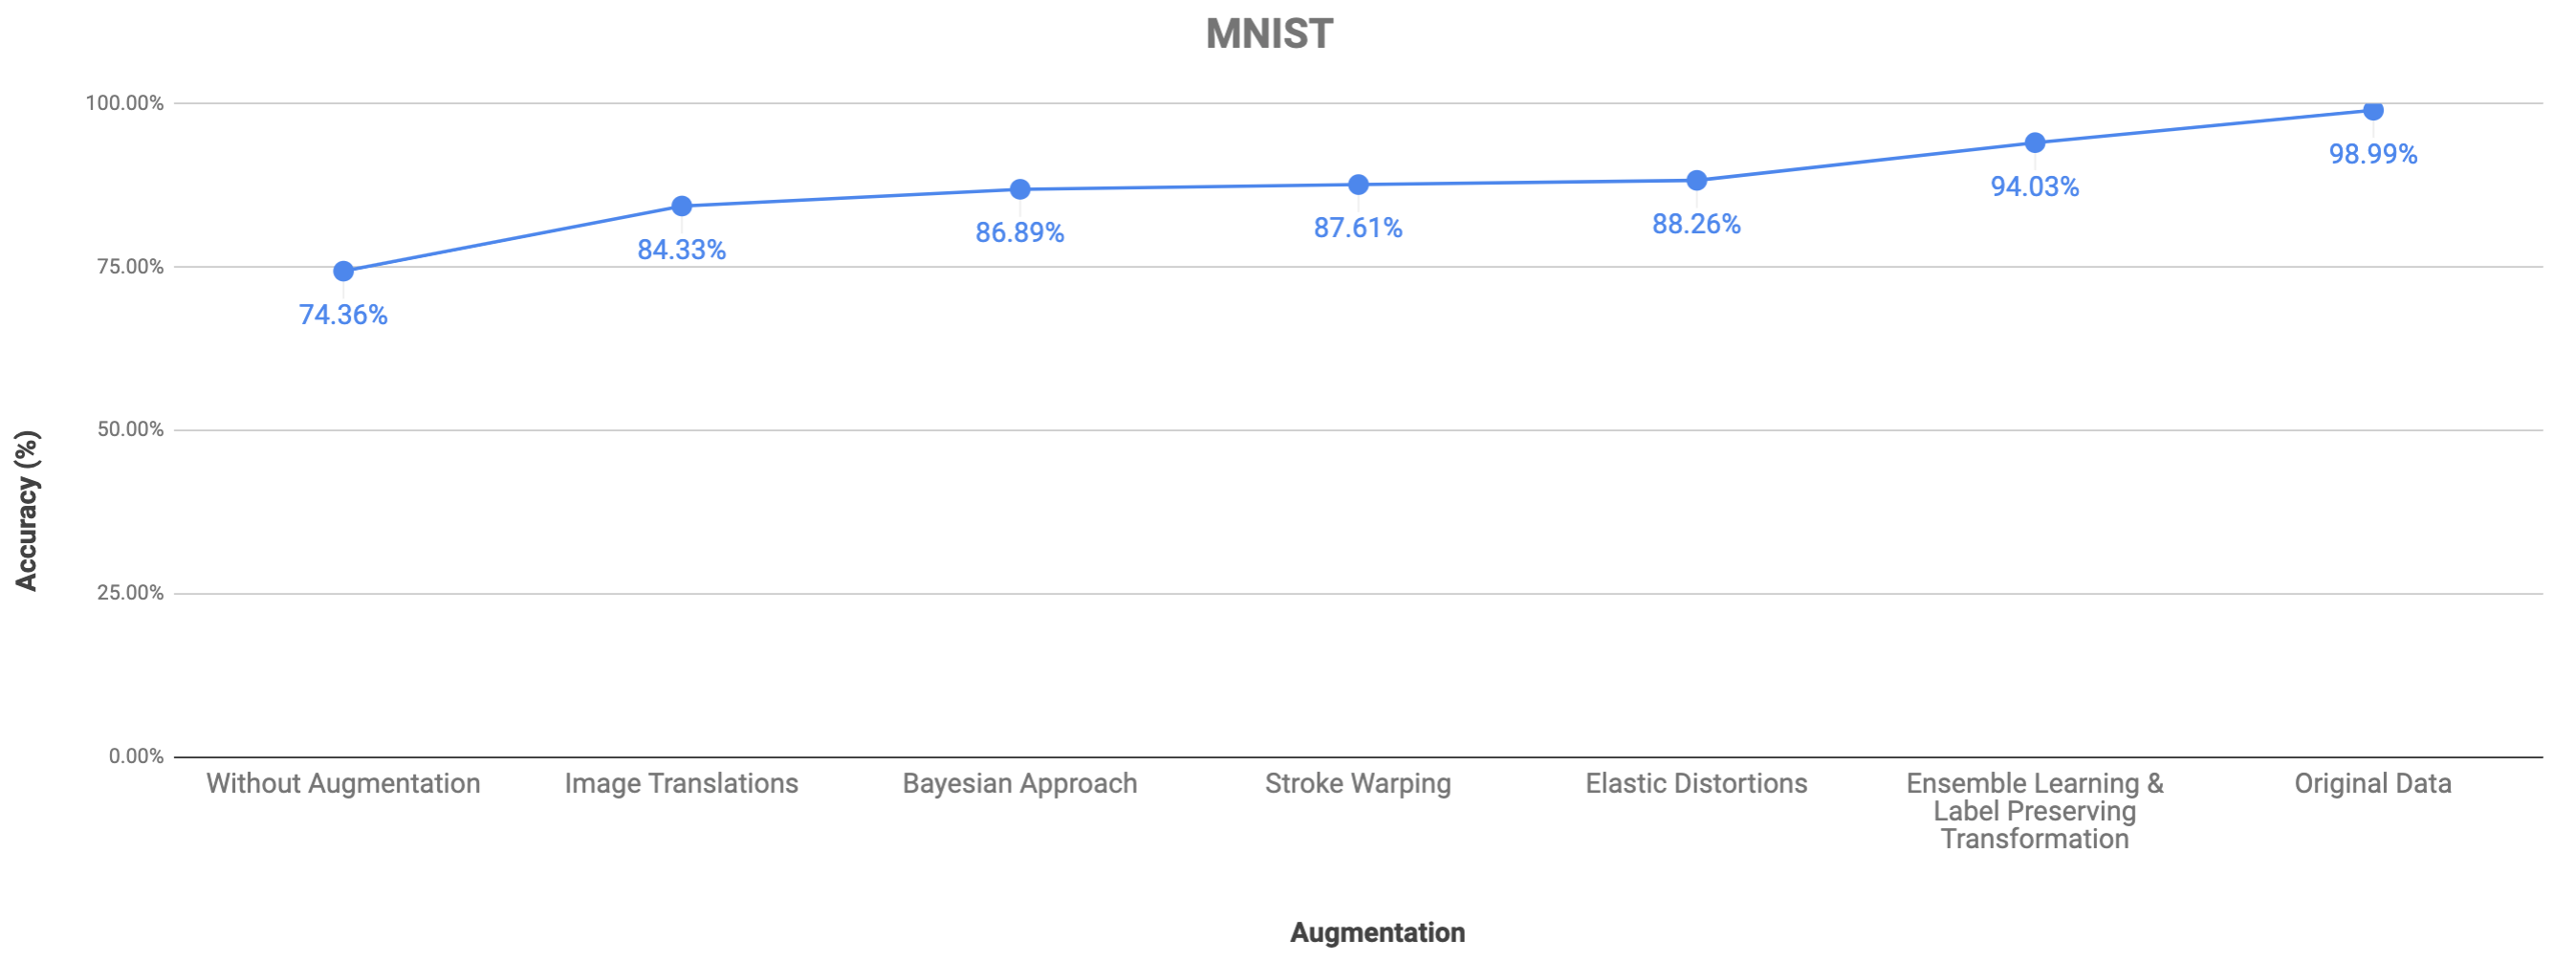
\includegraphics[width=1\textwidth]{fig/contribution/mnist-ensamble-result}
  \caption{Comparative result between Ensemble Learning \& Label Preserving Transformations augmentation and other augmentation techniques on MNIST dataset.}
\end{figure}


\begin{figure}
  \centering
  \label{fig:Fashion_MNIST_ensamble_result}
  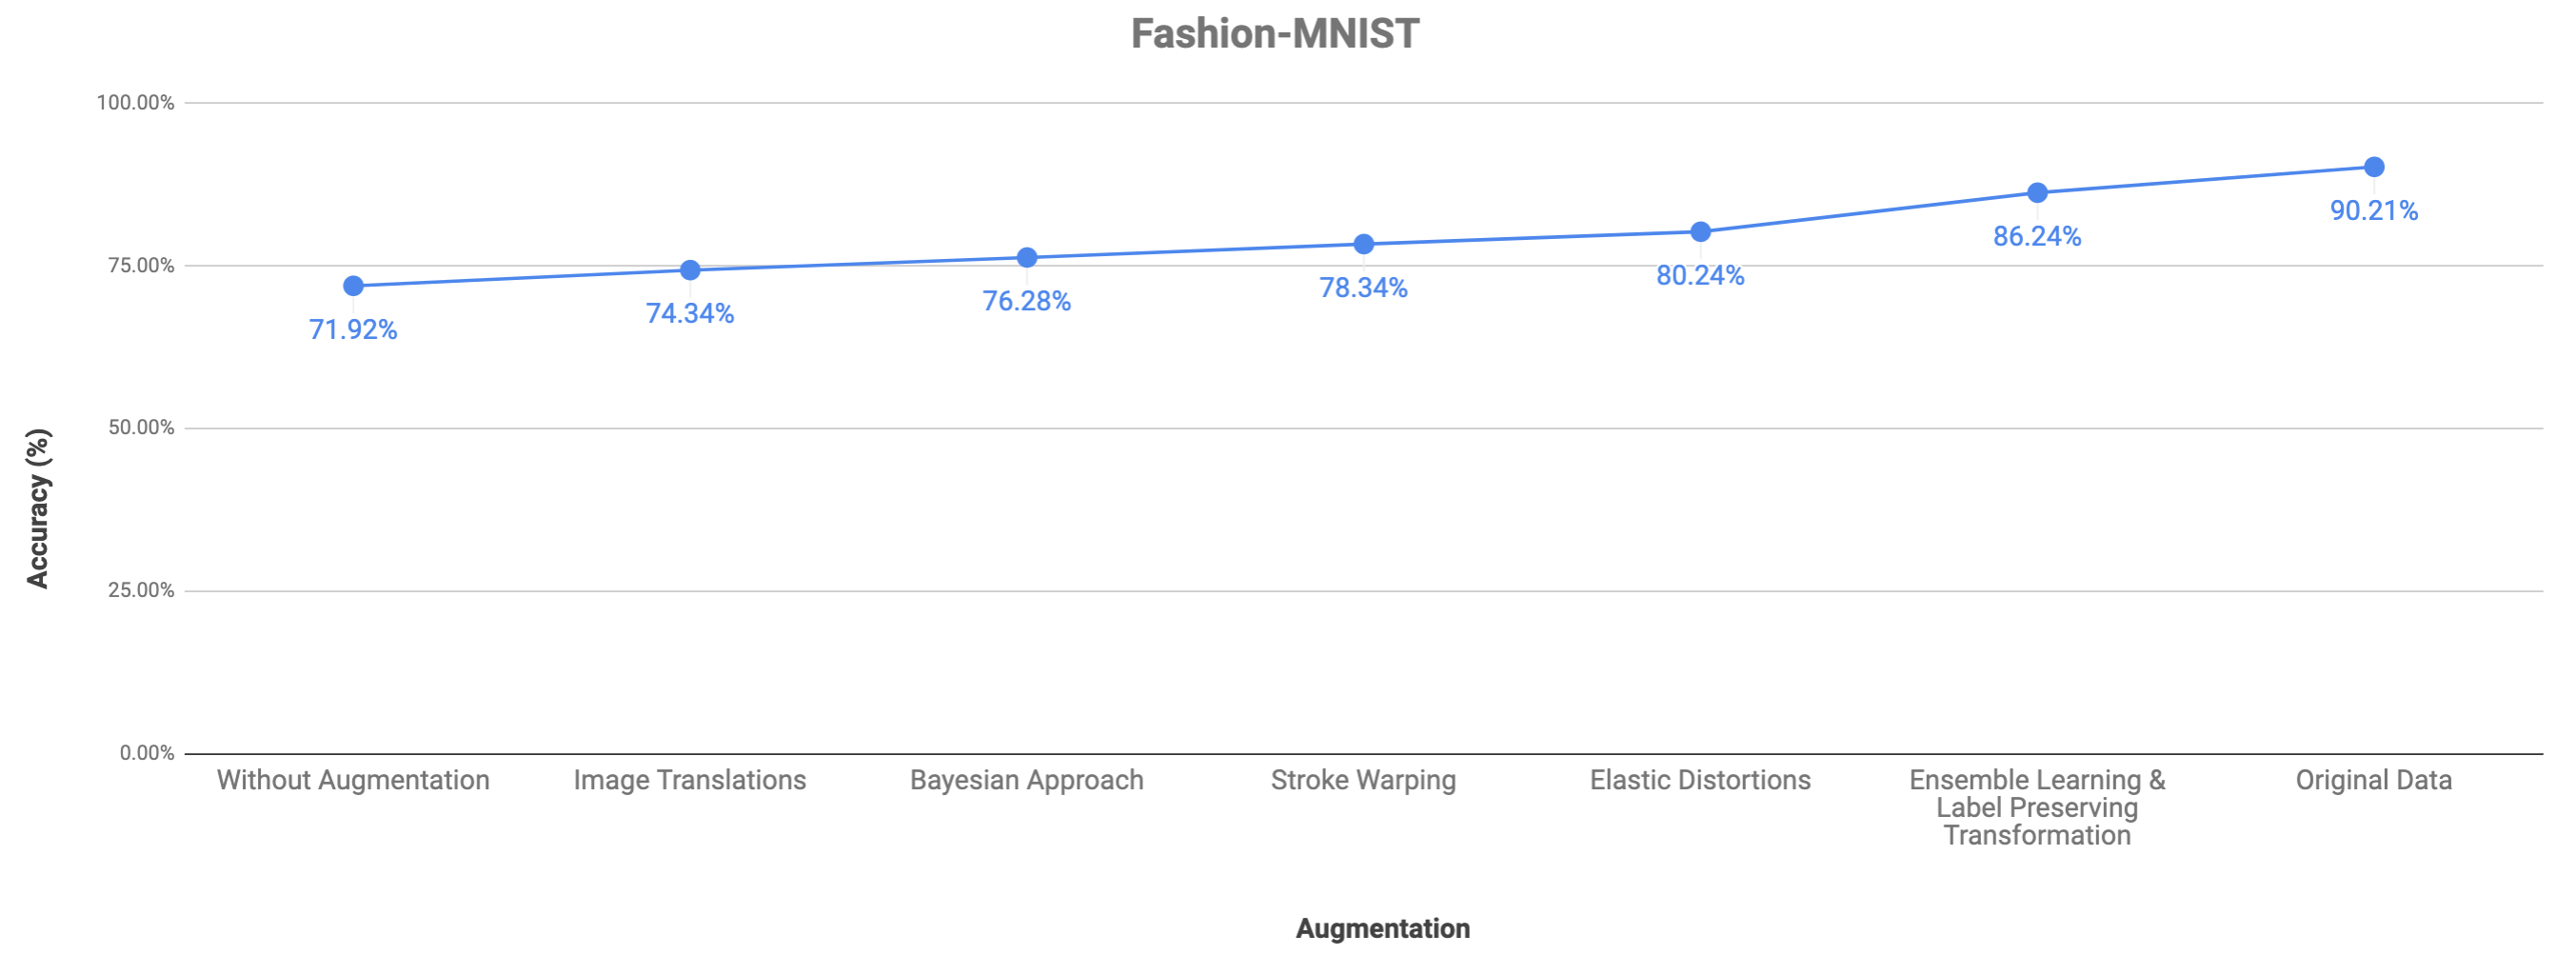
\includegraphics[width=1\textwidth]{fig/contribution/fashion-mnist-ensamble-result}
  \caption{Comparative result between Ensemble Learning \& Label Preserving Transformations augmentation and other augmentation techniques on Fashion-MNIST dataset.}
\end{figure}


\begin{figure}
  \centering
  \label{fig:Cifar_10_ensamble_result}
  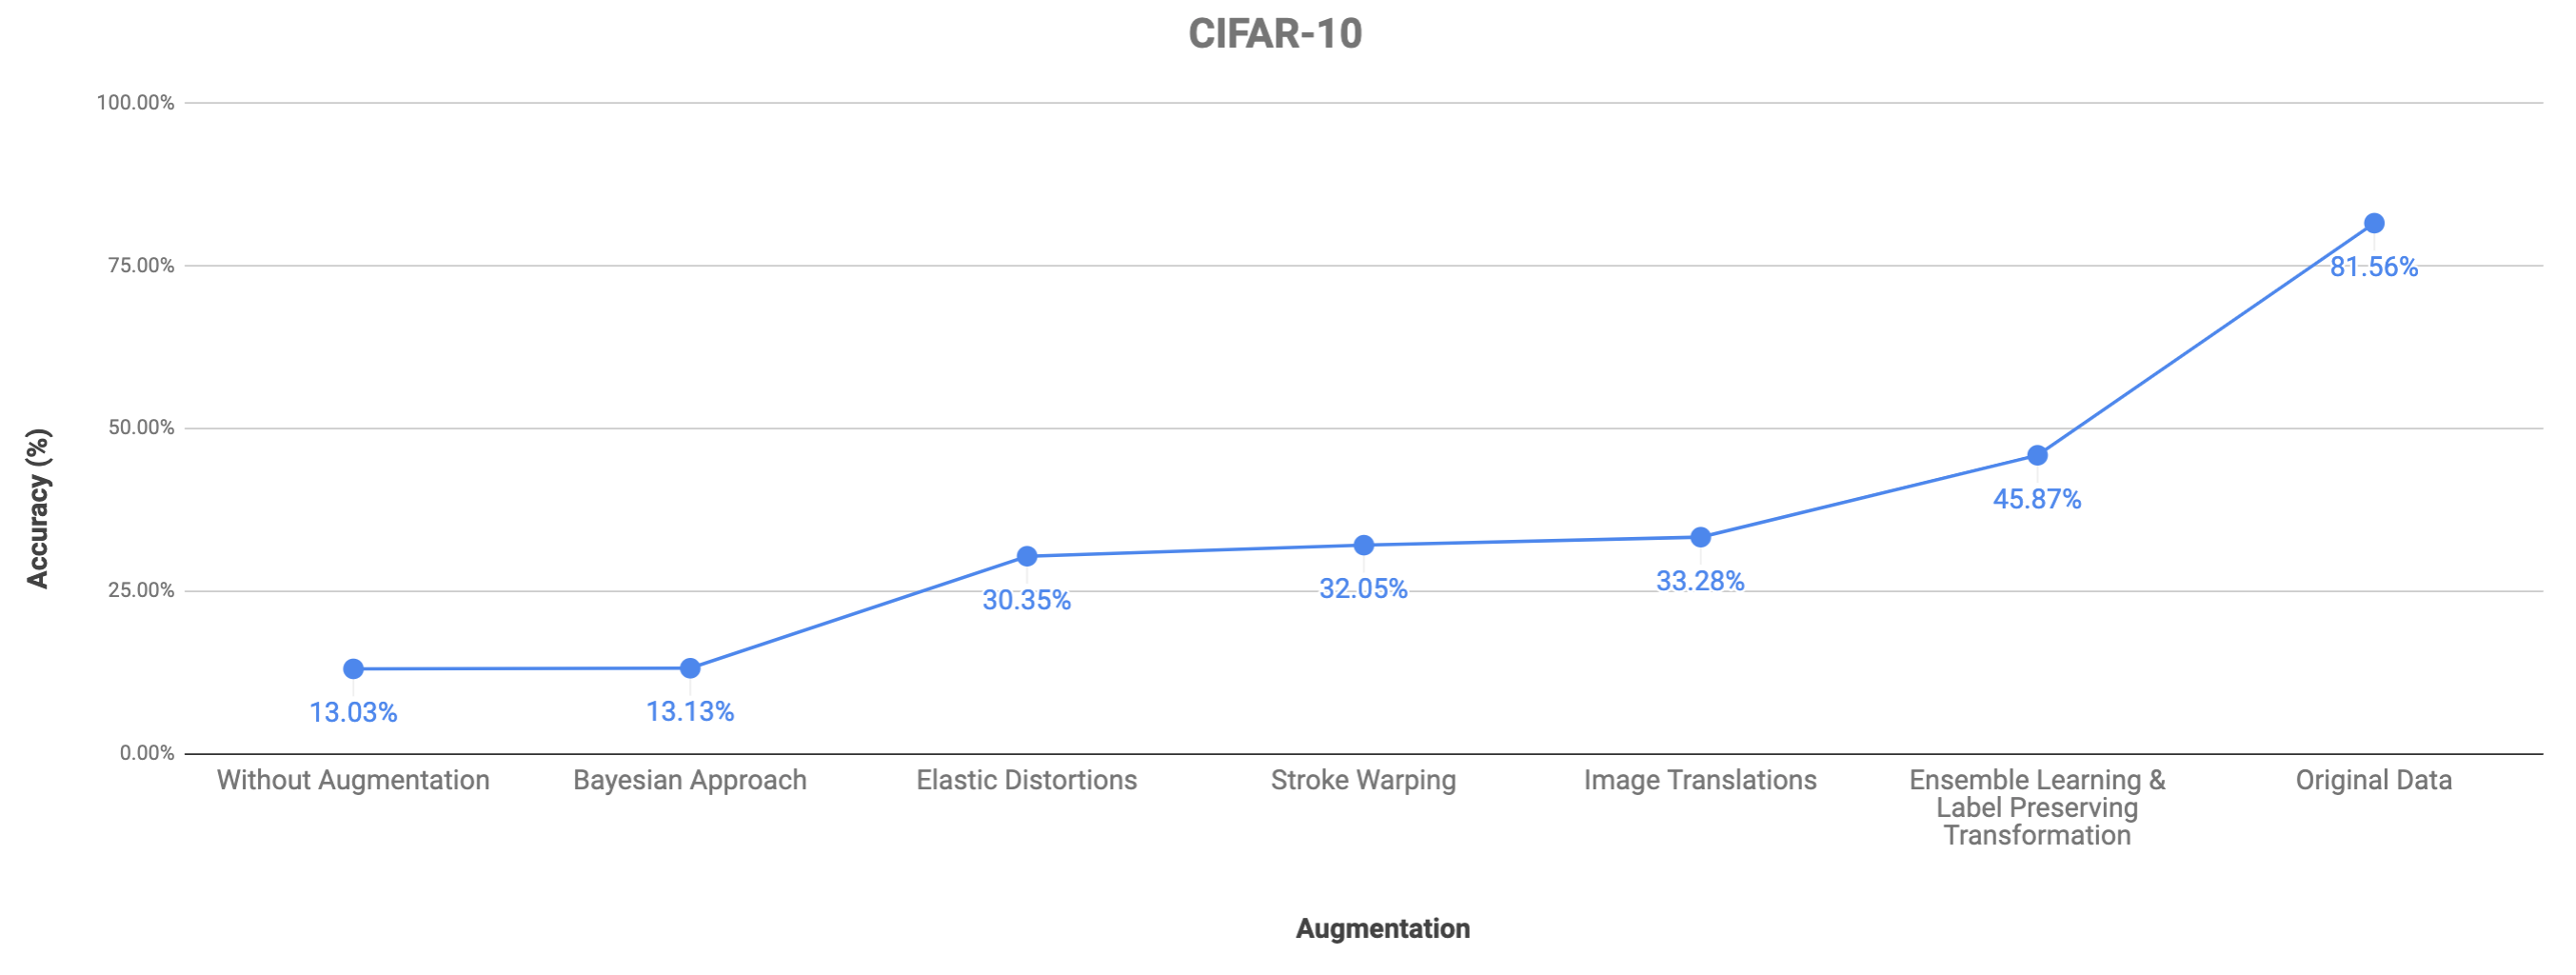
\includegraphics[width=1\textwidth]{fig/contribution/cifar-10-ensamble-result}
  \caption{Comparative result between Ensemble Learning \& Label Preserving Transformations augmentation and other augmentation techniques on CIFAR-10 dataset.}
\end{figure}

\begin{figure}
  \centering
  \label{fig:Fashion_MNIST_Ensamble_Heatmaps}
  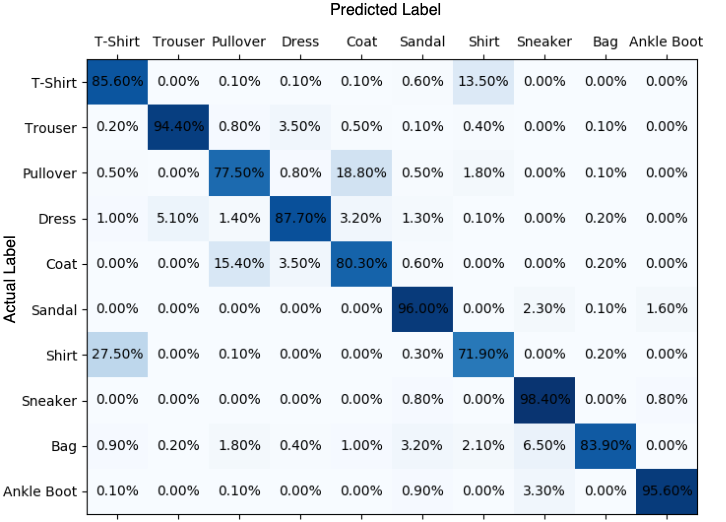
\includegraphics[width=1\textwidth]{fig/contribution/Fashion_MNIST_Ensamble}
  \caption{Prediction accuracy of each class on Fashion-MNIST for Ensemble Learning \& Label Preserving Transformations.}
\end{figure}

\section{Color Randomization \& Ensemble Learning}
As the name clearly indicates, this technique tackles the datasets such as Cifar-10 with RGB images.
As we have stated in Chapter \ref{tit:results} there is a significant gap between the accuracy of few-shot
learning and learning on original data for the Cifar-10 dataset. Further investigation on this
dataset made it obvious that the colors have been highly instrumental in learning. Figure \ref{fig:original_cifar_10}
presents the detailed accuracy of classes' prediction on the original data of Cifar-10. As it
demonstrates, for instance, many airplane samples mistakenly have been classified as a ship even on
the original dataset. It is trivial that CNN learns the colors and classifies the samples based on
that since there is no shape similarity between airplane and ship but they have almost the same
background-color (blue\footnote{Airplanes are almost have sky and ships have sea background}). In this technique, we approach to prevent unnecessary color learning such as background-color in the classifier with augmentation of the data with a random color.

\begin{figure}
  \centering
  \label{fig:original_cifar_10}
  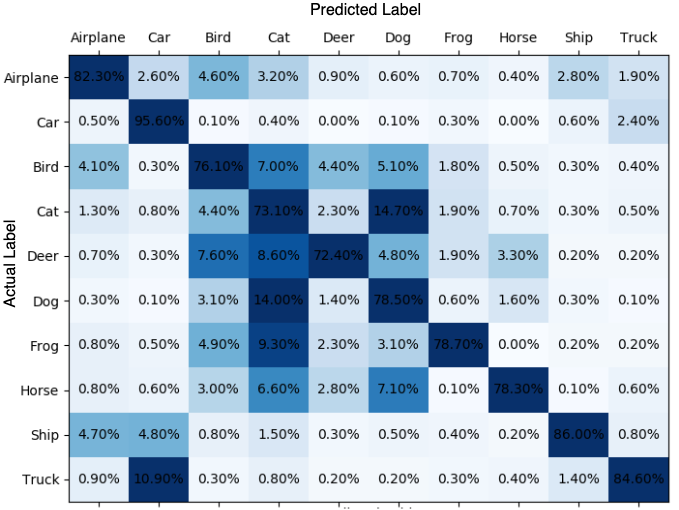
\includegraphics[width=1\textwidth]{fig/contribution/original_cifar_10}
  \caption{Prediction accuracy of each class on the original CIFAR-10 dataset.}
\end{figure}

In the first step, data will be augmented similar to the previous technique (Ensemble Learning \& Label Preserving Transformations). In the second step, images in the augmented dataset will be converted from the RGB color model to the HSI color model \cite{image-processing} as follows:

\begin{equation}
  \label{eq:hue}
  h=\left\{\begin{array}{ll}
    \theta \quad \quad \text { if } B \leq G & \text { with } \quad \theta=\cos ^{-1}\left\{\frac{1 /[(r-g)+(r-b)]}{\left[(r-g)^{2}+(r-b)(g-b)\right]^{1 / 2}}\right\} \\
    2 \pi-\theta \quad \text { otherwise }   &
  \end{array}\right\}
\end{equation}

Where $h$ represents the hue and $r,g$ , and $b$ denoted the normalized RGB value:

\begin{equation}
  r = \frac{R}{R+B+G} \ , \quad \quad b = \frac{B}{R+B+G} \ , \quad \quad g = \frac{G}{R+B+G}
\end{equation}


$s$ determines the saturation of color (Chroma) and is defined as follows:
\begin{equation}
  s=1-3 \cdot \min (r, g, b) ; \quad \mathbf{s} \in[0,1] \quad (\text{with exception for black with} \ (s=0) )
\end{equation}

$i$ determines the intensity and is defined as follows:
\begin{equation}
  i=(R+G+B) /(3 \cdot 255) ; \quad i \in[0,1]
\end{equation}

After converting the images to the HSI model, we will enlarge the dataset by a factor of four for each
image by randomizing the color of each sample. Color randomization adds a
random value between $\pi$ and $- \pi$ to the hue of the pixel mentioned in equation
(\ref{eq:hue}). The following equation presents the new hue denoted as $h'$ formally:
\begin{equation}
  \label{eq:new_hue}
  h'= h + random(\pi, - \pi)
\end{equation}

In the last step, we reconvert the augmented dataset to the RGB color model and start the learning
phase as before. The test and prediction phase will be accomplished exactly like the previous
technique.

\begin{figure}
  \centering
  \label{fig:cifar_10_random_color_result}
  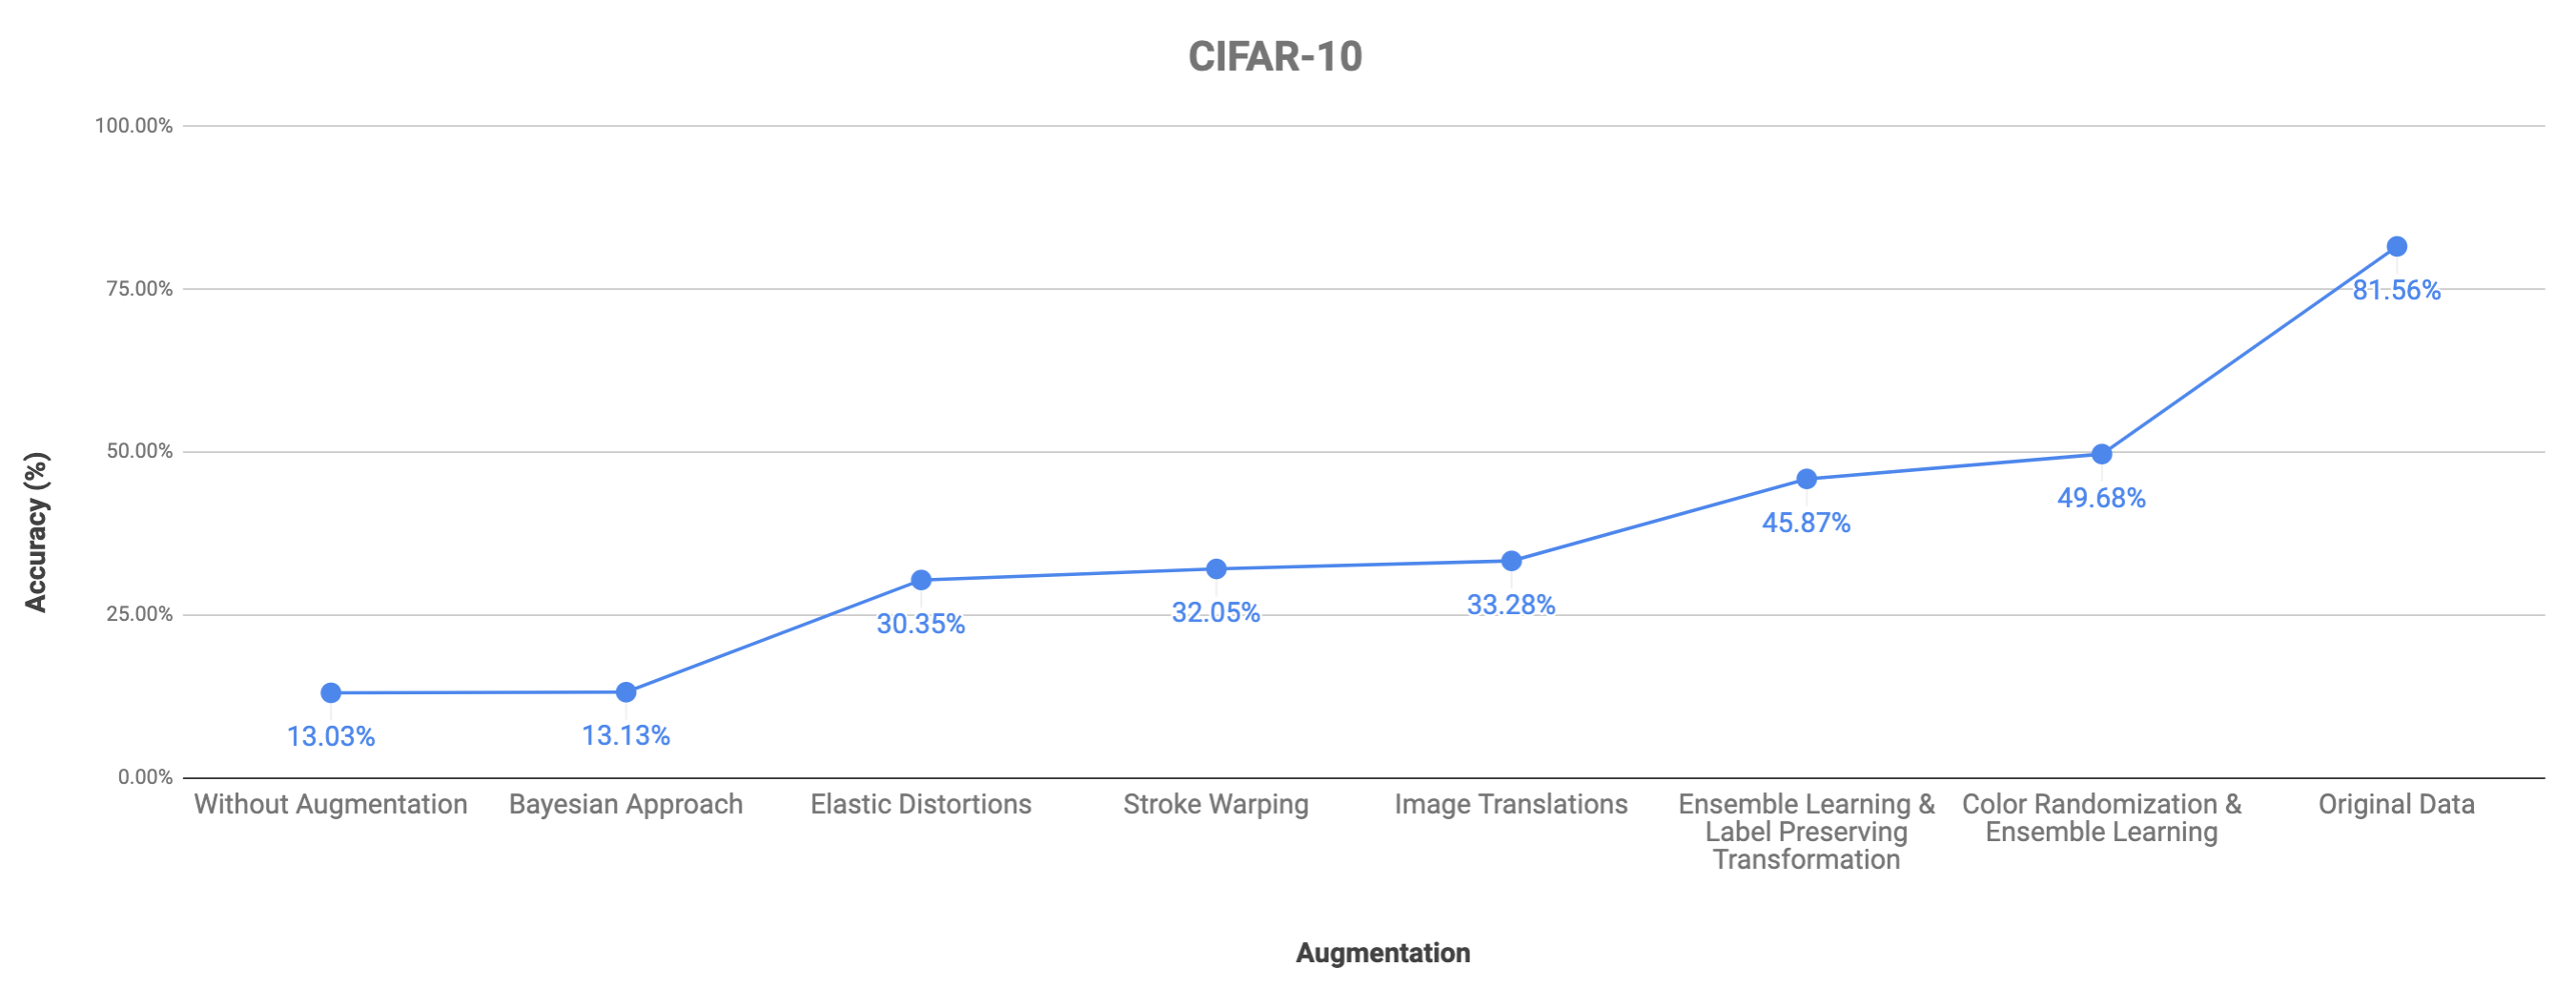
\includegraphics[width=1\textwidth]{fig/contribution/cifar-10-random-color-result}
  \caption{Comparative result between Color Randomization \& Ensemble Learning augmentation and other augmentation techniques on CIFAR-10 dataset.}
\end{figure}

We selected the HSI color model to randomize the color without the disadvantageous effect on the
pixel's intensity or chroma. As equation (\ref{eq:new_hue}) illustrates this matter our
technique only changes the hue of the pixels. It enables us not to only prevent the model from
unnecessary color learning but also not losing important information such as interest points,
edges, corners, and etc. in the picture. Figure \ref{fig:cifar_10_random_color_result} represents the result
of this technique on Cifar-10 besides other introduced techniques. It demonstrates that this
technique is even, better, than the previous one.


\section{Random Erasing \& Bayesian Approach}
Finally, we attempt to improve the bayesian approach with augmenting the
dataset at the beginning. It means that we augment our few-shot dataset before the bayesian approach
starts to generate synthetic data. The data augmentation will be carried out with an augmentation
technique called random erasing which is inspired by an introduced work by Zhun Zhong et al.
\cite{random_erasing}. In this technique for augmentation, we choose random patches smaller than
original images size in the dataset and erase them. We erase $100$ random patches with size $5
  \times 5$ from the images to augment our few-shot dataset with a factor of $100$. The influence of
such an augmentation with random erasing is similar to the dropout layer in CNNs \cite{dropout_book}.
Nevertheless, in the random erasing instead of disabling random nodes (random discrete pixels), an
area will be erased (disabled). Considering this augmentation, some negligible objects can be erased
from samples, therefore, it can improve accuracy and cause that the bayesian approach has a more
realistic and better estimation of class' distribution and observed posterior introduced in
equation (\ref{eq:observed-posterior}).

Figure \ref{fig:random_erasiong_result} represents a comparison between the bayesian approach with
and without random erasing. It demonstrates that this technique does not only  achieve better
performance and accuracy on all introduced datasets in theory, but also pragmatically.


\begin{figure}
  \centering
  \label{fig:random_erasiong_result}
  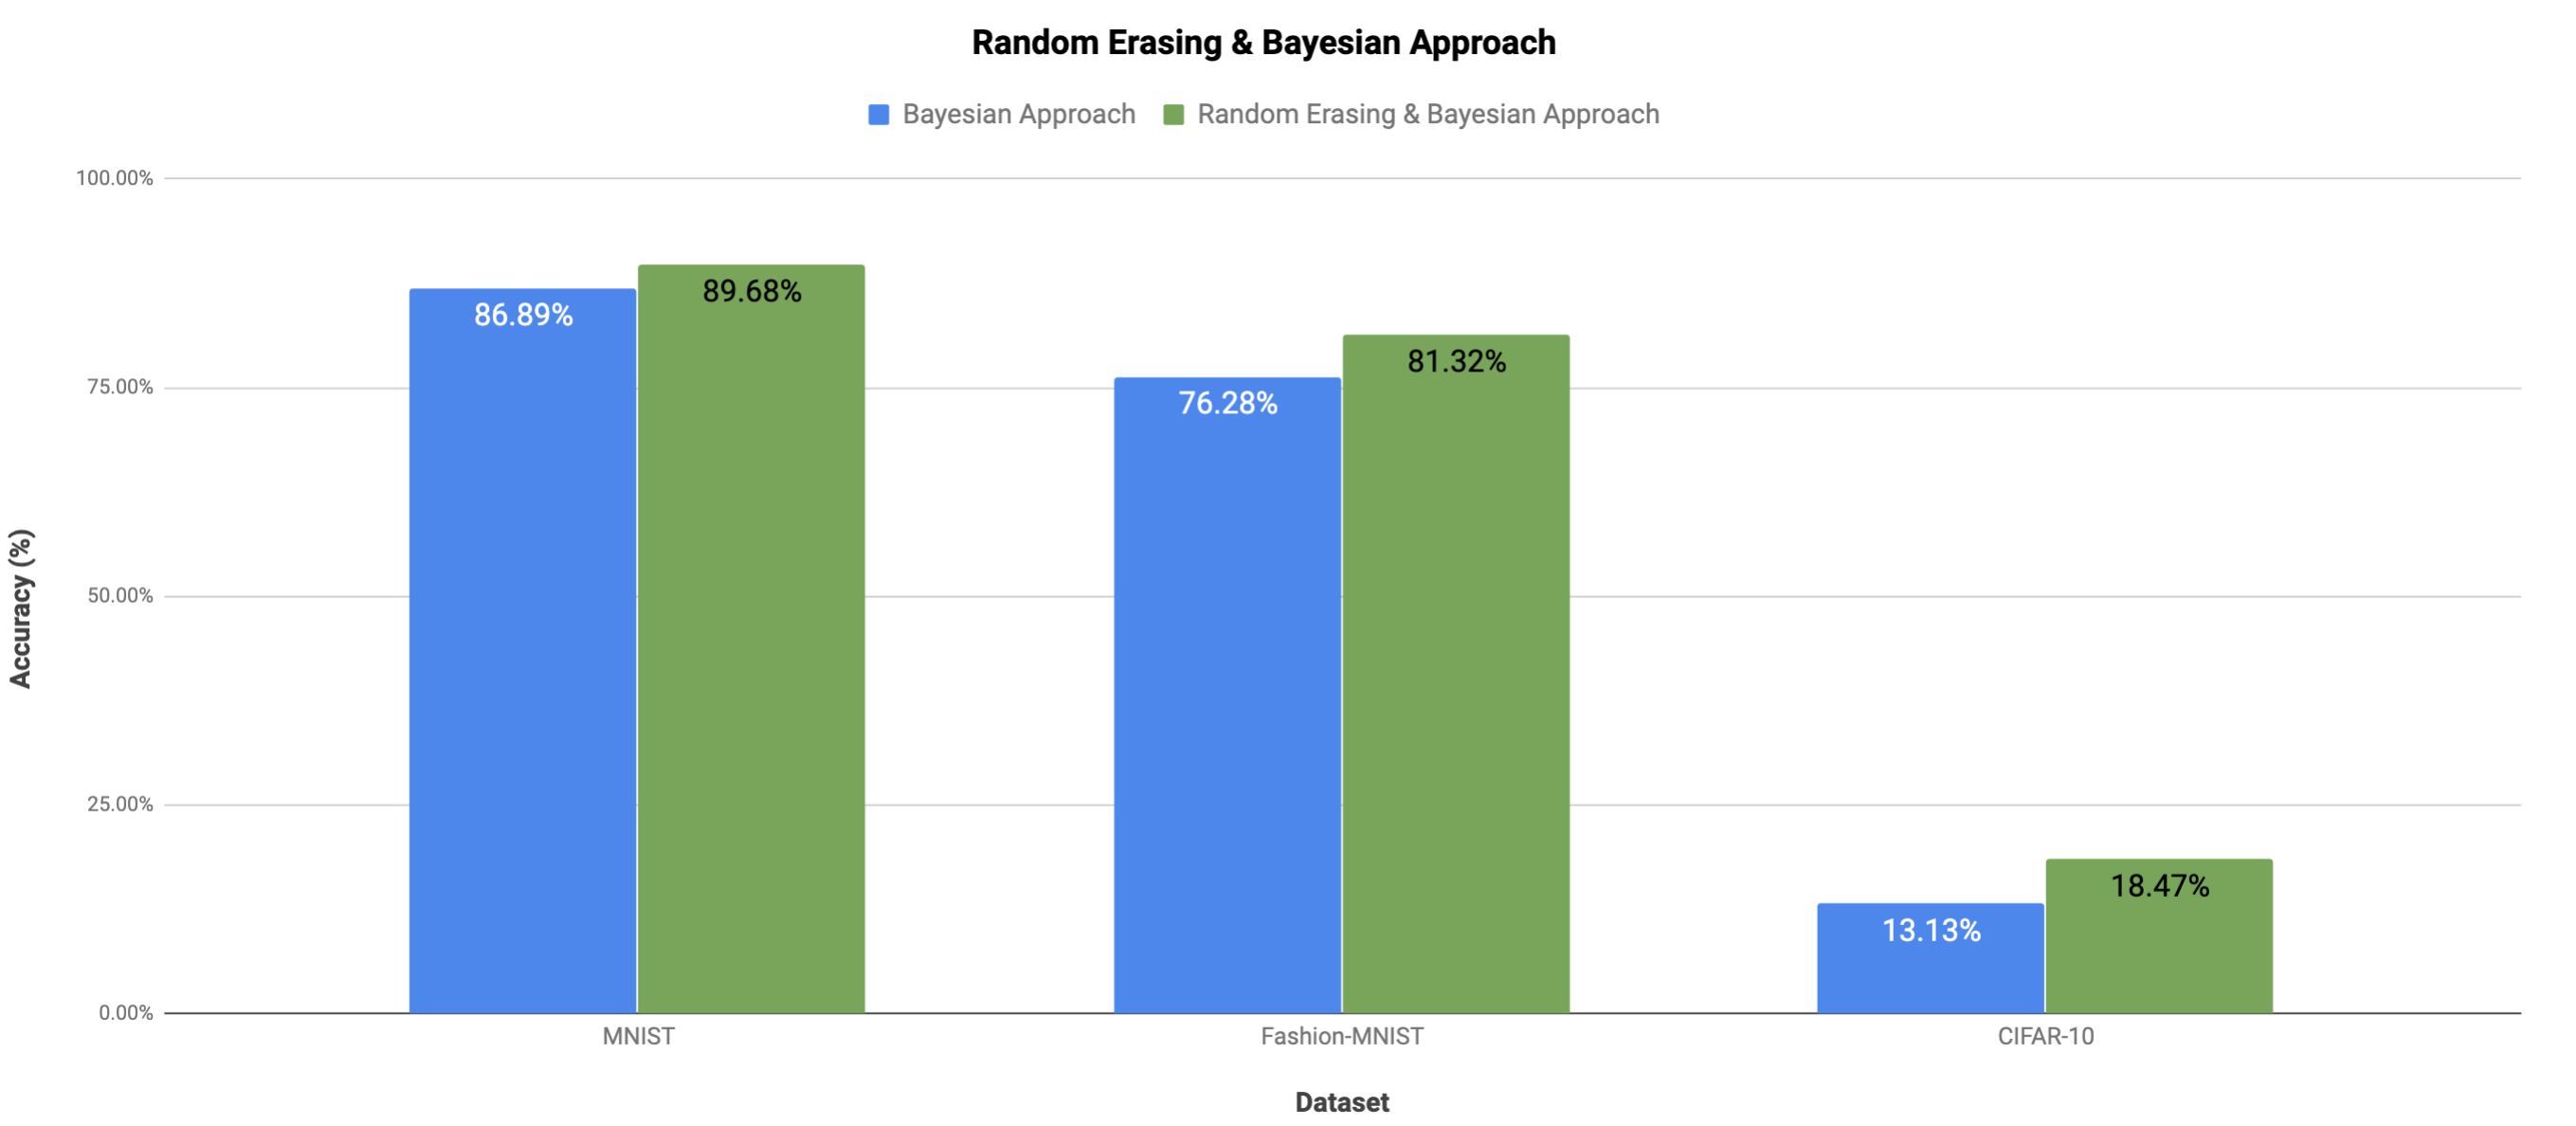
\includegraphics[width=1\textwidth]{fig/contribution/random-erasing-result}
  \caption{Comparative result between Bayesian Approach with and without random erasing.}
\end{figure}

\chapter{Conclusion}

\begin{table}[]
  \label{all_results}
  \resizebox{\textwidth}{!} & 71.92\%                                     & 13.03\%                                \\ \hline
      \textbf{Image Translations}                  & \multicolumn{1}{c|}{84.33\%} & 74.34\%                                     & 33.28\%                                \\ \hline
      \textbf{Elastic Distortions}                 & \multicolumn{1}{c|}{88.26\%} & 80.24\%                                     & 30.35\%                                \\ \hline
      \textbf{Stroke Warping}                      & 87.61\%                      & 78.34\%                                     & 32.05\%                                \\ \hline
      \textbf{Bayesian Approach}                   & 86.89\%                      & 76.28\%                                     & 13.13\%                                \\ \hline
      \textbf{\begin{tabular}[c]{@{}l@{}}Ensemble Learning \&\\ Label Preserving Transformation\end{tabular}}          & 94.03\%                      & 86.24\%                                     & 45.87\%                                \\ \hline
      \textbf{\begin{tabular}[c]{@{}l@{}}Color Randomization \&\\ Ensemble Learning\end{tabular}}          & \multicolumn{1}{c|}{-}       & -                                           & 49.68\%                                \\ \hline
      \textbf{\begin{tabular}[c]{@{}l@{}}Random Erasing \&\\ Bayesian Approach\end{tabular}}          & 89.68\%                      & 81.32\%                                     & 18.47\%                                \\ \hline
    \end{tabular}%
  }
  \caption{Accuracy of each data augmentation technique on each 10-shot dataset.}
\end{table}


In this work, we have dealt with few-shot learning. First of all, we introduced data augmentation
that helps to reach better accuracy and prevent overfitting for few-shot learning. After that, we
introduce several well-known approaches and techniques of data augmentation that with different
deformations and transformations on images augment the few-shot datasets.  In the next step, we
implemented all approaches and techniques on several datasets. The implementation helped us to
obtain pragmatic results of each approach and technique on each dataset. These results helped us to
have a comprehensive comparison of the performance of each approach and technique and exposed the
advantages and disadvantages of them in different circumstances. The comparison showed us that the
approaches and techniques have different performance on different datasets. In the end, based on the
comparison and advantages and disadvantages of each approach and technique we proposed three new
techniques with a combination of inspired by other works and introduced approaches and techniques in
this work. These new techniques reached a better and robust performance and accuracy on different
datasets. Table \ref{all_results} shows all results of data augmentation approaches and techniques introduced
and mentioned in this work.


With this work, we hope to have highlighted solutions of low accuracy and overfitting in few-shot learning and that this work can help the research community to increase the accuracy in few-shot learning on any image datasets.